\documentclass[12pt,letter]{article}
\usepackage{../downey_format}


%\usepackage{tikz}
%\usetikzlibrary{arrows.meta,shapes.geometric}
%\usetikzlibrary{arrows.meta}

\begin{document}
	
	% set the section number, along with figure and equation numbers
	\setcounter{section}{7}	
	\setcounter{figure}{\thesection}   
	\renewcommand\thefigure{\thesection.\arabic{figure}}
	\setcounter{equation}{\thesection}   
	\renewcommand\theequation{\thesection.\arabic{equation}}

\section{Clustering}

Clustering groups observations that ``look similar'' without using any external labels. In contrast to classification, where each sample is mapped to a known class, clustering is unsupervised---the algorithm must discover structure on its own. Figure~\ref{fig:Clustering} illustrates this distinction: the left panel shows a labeled decision surface learned from annotated data (classification), while the right panel shows the same points partitioned solely by proximity, with no labels supplied (clustering). Clustering is valuable when you 
\begin{enumerate}
\item have no ground-truth labels
\item suspect there are hidden sub-populations
\item want a quick exploratory summary before choosing a supervised model.
\end{enumerate}

\begin{data}
\textbf{Wine Dataset}

\noindent The wine dataset contains 178 samples of Italian red wine from three cultivars grown in the same region. Each sample is represented by 13 continuous measurements, such as alcohol content, flavonoid concentration, magnesium level, and color intensity. These measurements capture chemical and physical differences among the wines. Since the three cultivars form natural but partially overlapping groups, the wine dataset is commonly used as a benchmark for clustering and other multivariate analysis methods.

\begin{figure}[H]
    \centering
    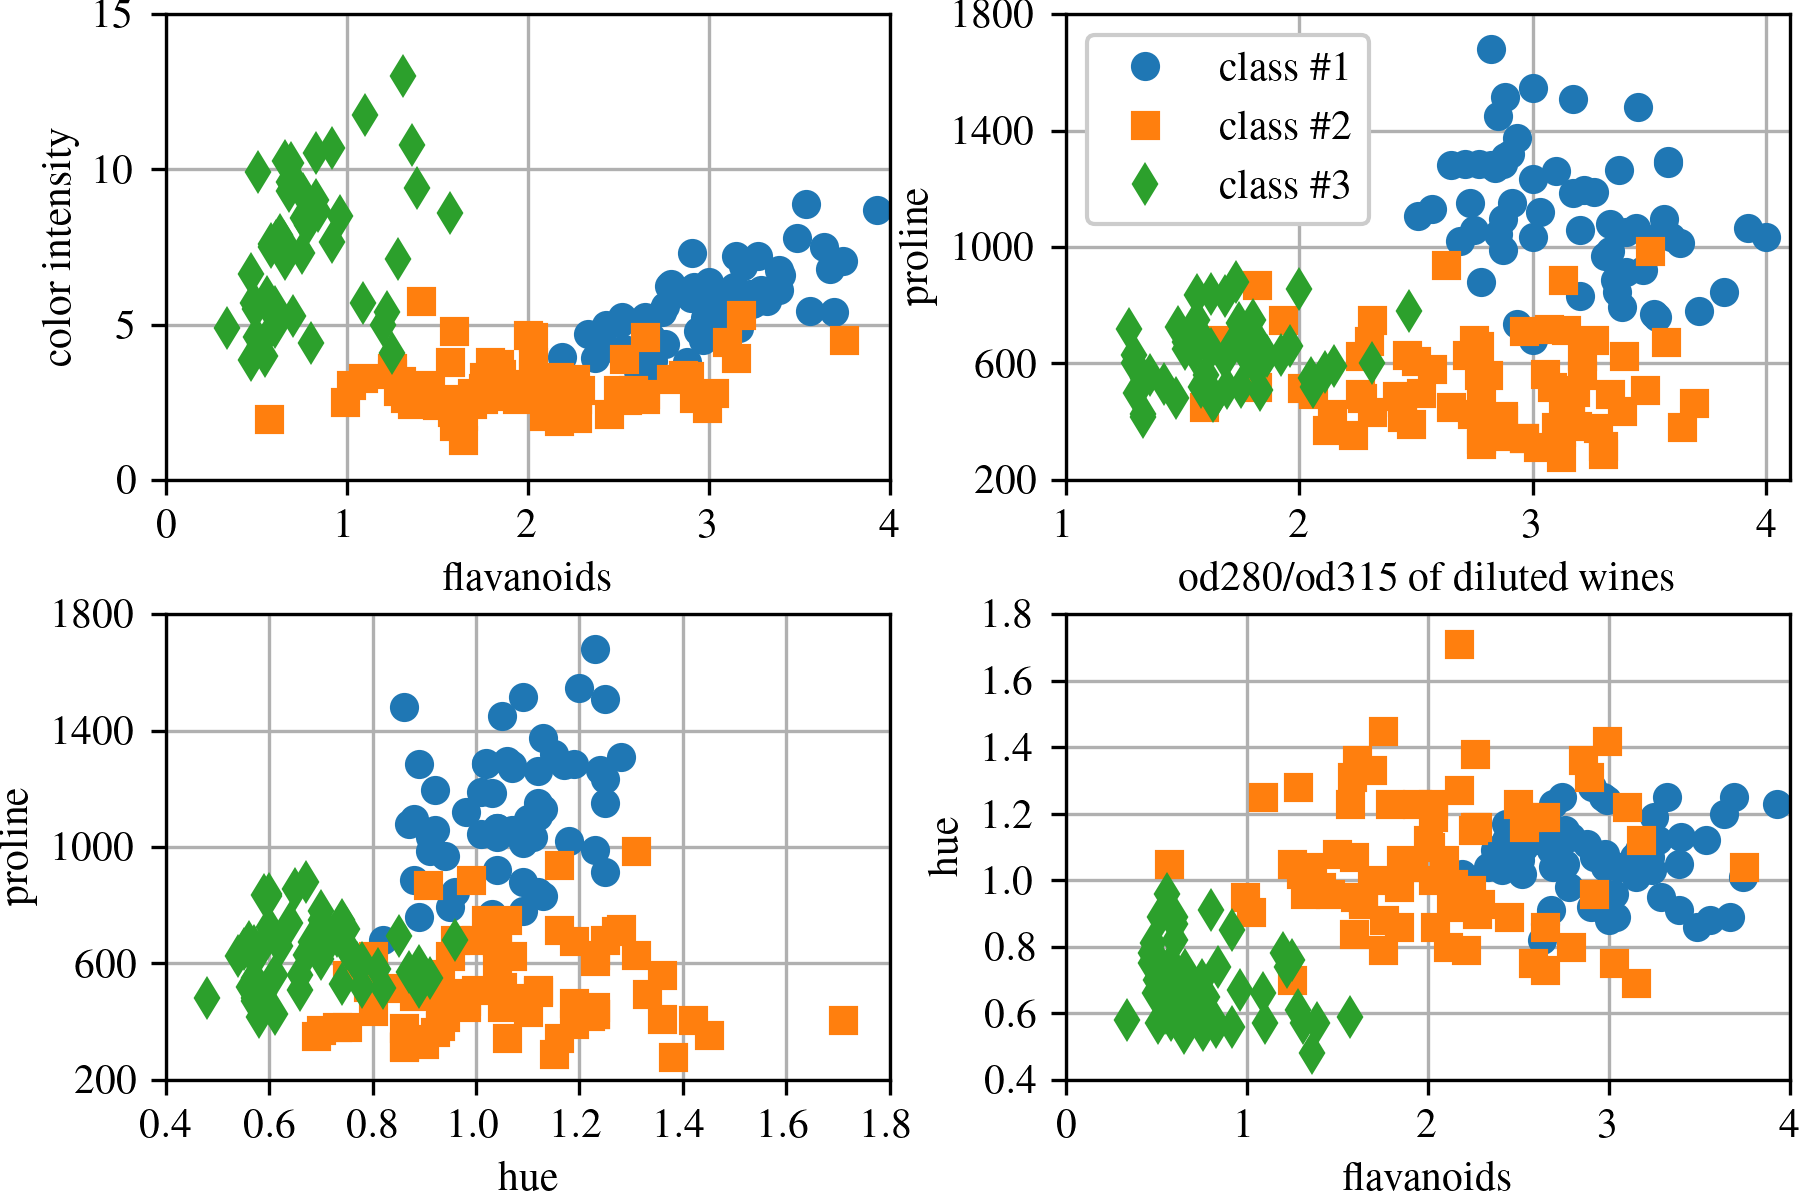
\includegraphics[width=5.6in]{../figures/wine_data_feature-feature.png}
    \caption{Two feature-feature plots developed for the wine data set.}
    \label{fig:MNIST_data_set}
\end{figure}
\end{data}


A clustering algorithm receives only the feature matrix
\begin{equation}
    X = \left[\mathbf{x}_1,\mathbf{x}_2,\ldots,\mathbf{x}_n\right]^\top,
\end{equation}
where each observation \(\mathbf{x}_i \in \mathbb{R}^d\) is described by \(d\) measured or engineered features. Unlike supervised learning, there is no target vector \(\mathbf{y}\) that tells the algorithm the correct answer. The goal is therefore not to reproduce known labels, but to discover structure that may be useful for interpretation, visualization, preprocessing, or later supervised modeling.

The word ``similar'' is important. Most clustering algorithms depend on a distance or similarity measure, such as Euclidean distance,
\begin{equation}
    d\left(\mathbf{x}_i,\mathbf{x}_j\right)
    =
    \left\lVert \mathbf{x}_i-\mathbf{x}_j \right\rVert_2.
\end{equation}
If one feature has a much larger numerical range than the others, it can dominate the distance calculation. For this reason, clustering is usually applied after feature scaling, particularly when the features have different units. In scikit-learn this is commonly handled by placing a transformer such as \texttt{StandardScaler} before the clustering estimator in a pipeline.

\begin{figure}[H]
	\centering
	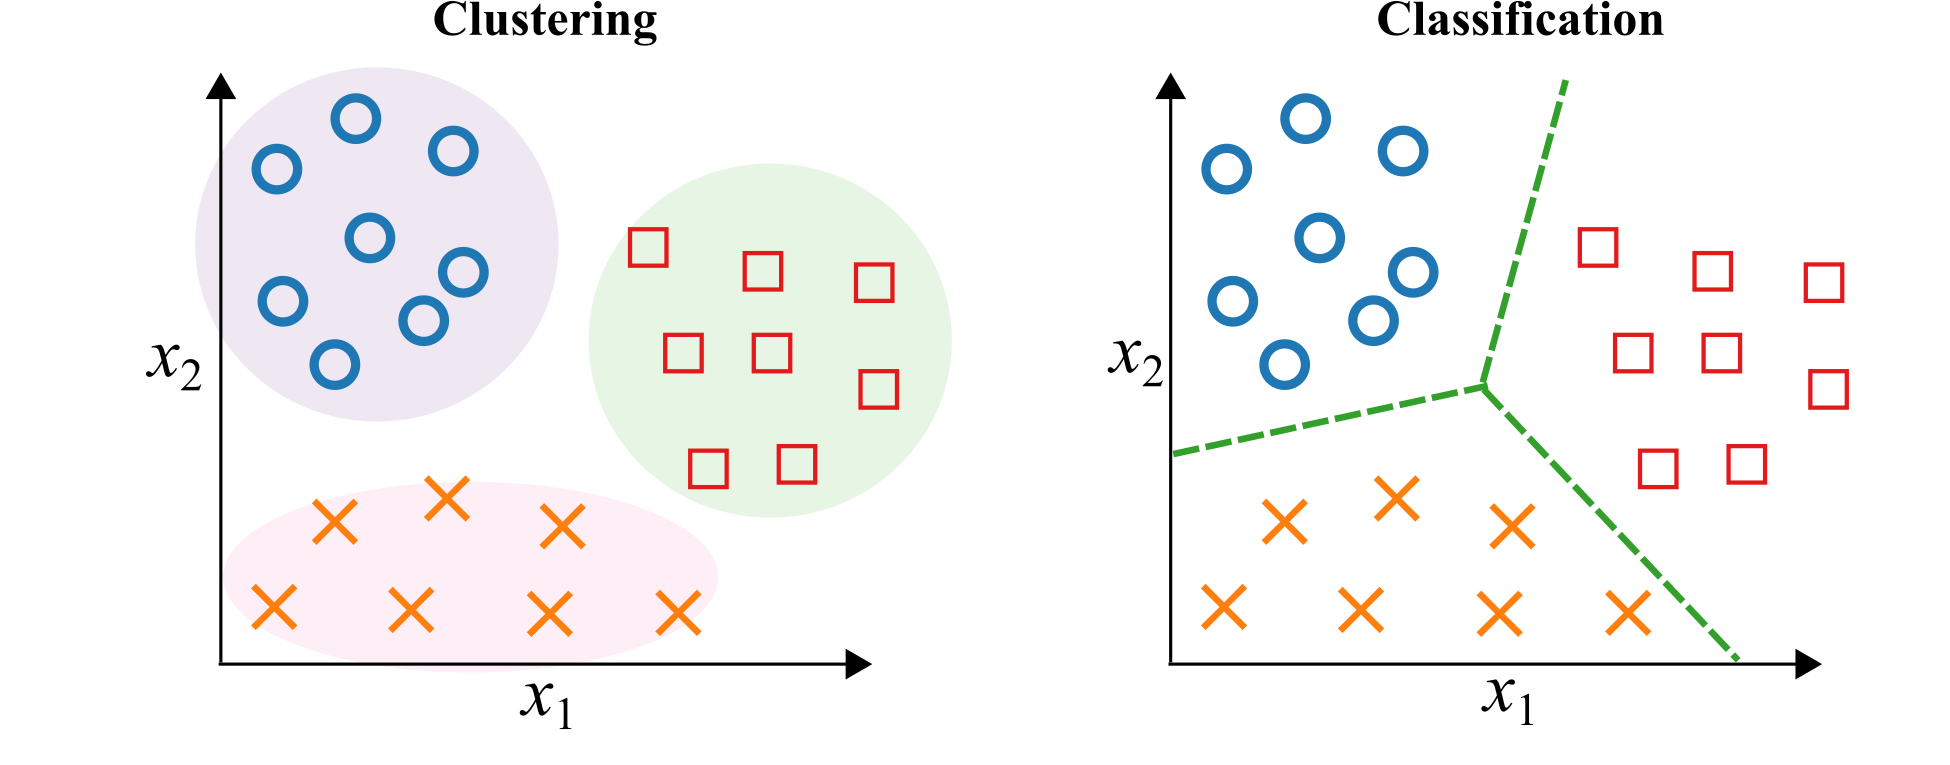
\includegraphics[width=6.5in]{../figures/Clustering_vs_Classification}
	\caption{A comparison between clustering on the left and classification on the right. }
	\label{fig:Clustering}
\end{figure}

Figure~\ref{fig:Clustering_methods} summarizes several common clustering ideas. The methods in this chapter differ mainly in how they define a cluster. K-means represents each cluster by a centroid. Hierarchical clustering builds a tree of nested groups. DBSCAN and HDBSCAN define clusters as dense regions separated by sparse regions. Gaussian mixture models treat the data as being generated by a weighted combination of probability distributions. These different assumptions lead to different strengths and weaknesses.

\begin{figure}[H]
	\centering
	
\includegraphics[width=6.5in]{../figures/Clustering_methods}
	\caption{Examples of several clustering methods.}
	\label{fig:Clustering_methods}
\end{figure}

\subsection{K-Means}
\label{subsec:kmeans}

K-means is one of the most widely used clustering algorithms. It partitions a data set into a chosen number of clusters, \(k\), by assigning each observation to the closest cluster center. Each cluster center is called a centroid because it is computed as the mean location of all observations assigned to that cluster. In scikit-learn, this model is implemented by \texttt{sklearn.cluster.KMeans}.

K-means is simple, fast, and easy to interpret. Its main assumption is that each cluster can be represented well by a single center and that points should be grouped by Euclidean distance from those centers. This works well for compact, roughly circular or spherical clusters. It works less well when clusters are curved, elongated, strongly overlapping, or have very different densities.

Throughout this section, the examples use the wine data set represented by two standardized features:
\[
    x_1 = \texttt{color\_intensity},
    \qquad
    x_2 = \texttt{proline}.
\]
The original wine data set includes three known wine classes. These class labels are useful for visualization, but they are not used by K-means. K-means only sees the feature values and tries to find groups based on distance.

\begin{figure}[H]
	\centering
	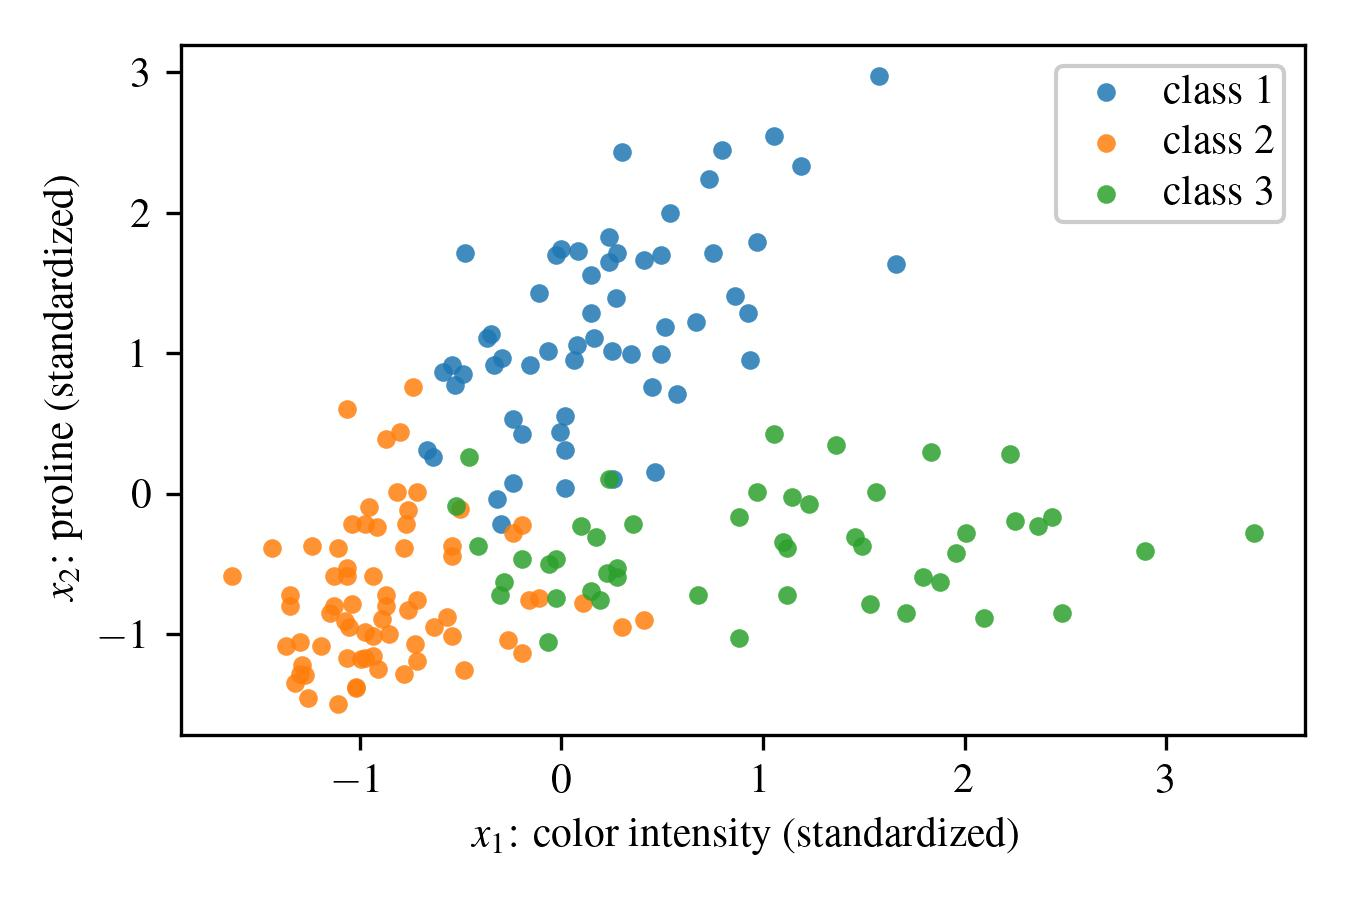
\includegraphics[width=4.5in]{../figures/K-means_wine_data.jpg}
	\caption{Wine data represented using two standardized features: color intensity and proline. Points are colored by the known wine class labels. These labels are shown only for interpretation and are not provided to K-means during clustering.}
	\label{fig:kmeans-wine-data}
\end{figure}

\subsubsection{Objective Function}

\paragraph{Problem setup}%
Given observations
\[
    X=\{\mathbf{x}_1,\mathbf{x}_2,\dots,\mathbf{x}_n\}
    \subset \mathbb{R}^d,
\]
K-means seeks \(k\) centroids
\[
    \boldsymbol{\mu}_1,\boldsymbol{\mu}_2,\dots,\boldsymbol{\mu}_k
\]
and cluster assignments
\[
    c_i \in \{1,2,\dots,k\}
\]
that minimize the within-cluster sum of squared distances:
\begin{equation}
    J
    =
    \sum_{i=1}^{n}
    \left\lVert
    \mathbf{x}_i-\boldsymbol{\mu}_{c_i}
    \right\rVert^2 .
    \label{eq:kmeans_objective}
\end{equation}

The objective \(J\) is often called the inertia or within-cluster sum of squares. A small value of \(J\) means that points are close to the centroids of their assigned clusters. Therefore, minimizing \(J\) encourages compact clusters.

The cluster label \(c_i\) is just an index. It does not necessarily correspond to a physical class label. For example, a K-means cluster labeled ``cluster 1'' does not automatically mean ``wine class 1.'' The cluster numbers are arbitrary and can change depending on the initialization.

\subsubsection{Assignment and Update Steps}

The most common optimization procedure for K-means is Lloyd's algorithm. It alternates between two simple steps: assign points to the nearest centroid, then update each centroid to the mean of the points assigned to it.

\begin{enumerate}
    \item \textbf{Initialize the centroids.} Choose \(k\) starting centroids, often randomly or using the k-means++ initializer.

    \item \textbf{Assignment step.} Assign each point to its closest centroid:
    \begin{equation}
        c_i
        =
        \arg\min_{j \in \{1,\dots,k\}}
        \left\lVert
        \mathbf{x}_i-\boldsymbol{\mu}_j
        \right\rVert^2 .
        \label{eq:kmeans_assignment}
    \end{equation}

    \item \textbf{Update step.} Recompute each centroid as the average of the points assigned to it:
    \begin{equation}
        \boldsymbol{\mu}_j
        =
        \frac{1}{|C_j|}
        \sum_{i:c_i=j}
        \mathbf{x}_i ,
        \label{eq:kmeans_update}
    \end{equation}
    where \(C_j\) is the set of points assigned to cluster \(j\).

    \item \textbf{Repeat.} Continue alternating between the assignment and update steps until the assignments stop changing or the decrease in \(J\) becomes very small.
\end{enumerate}

The assignment step divides the feature space into regions. Every point in one region is closer to one centroid than to the others. These regions are called Voronoi cells or decision regions. Figure~\ref{fig:kmeans-decision-regions} shows the final decision regions for K-means with \(k=3\) on the two-dimensional wine data.

\begin{figure}[H]
	\centering
	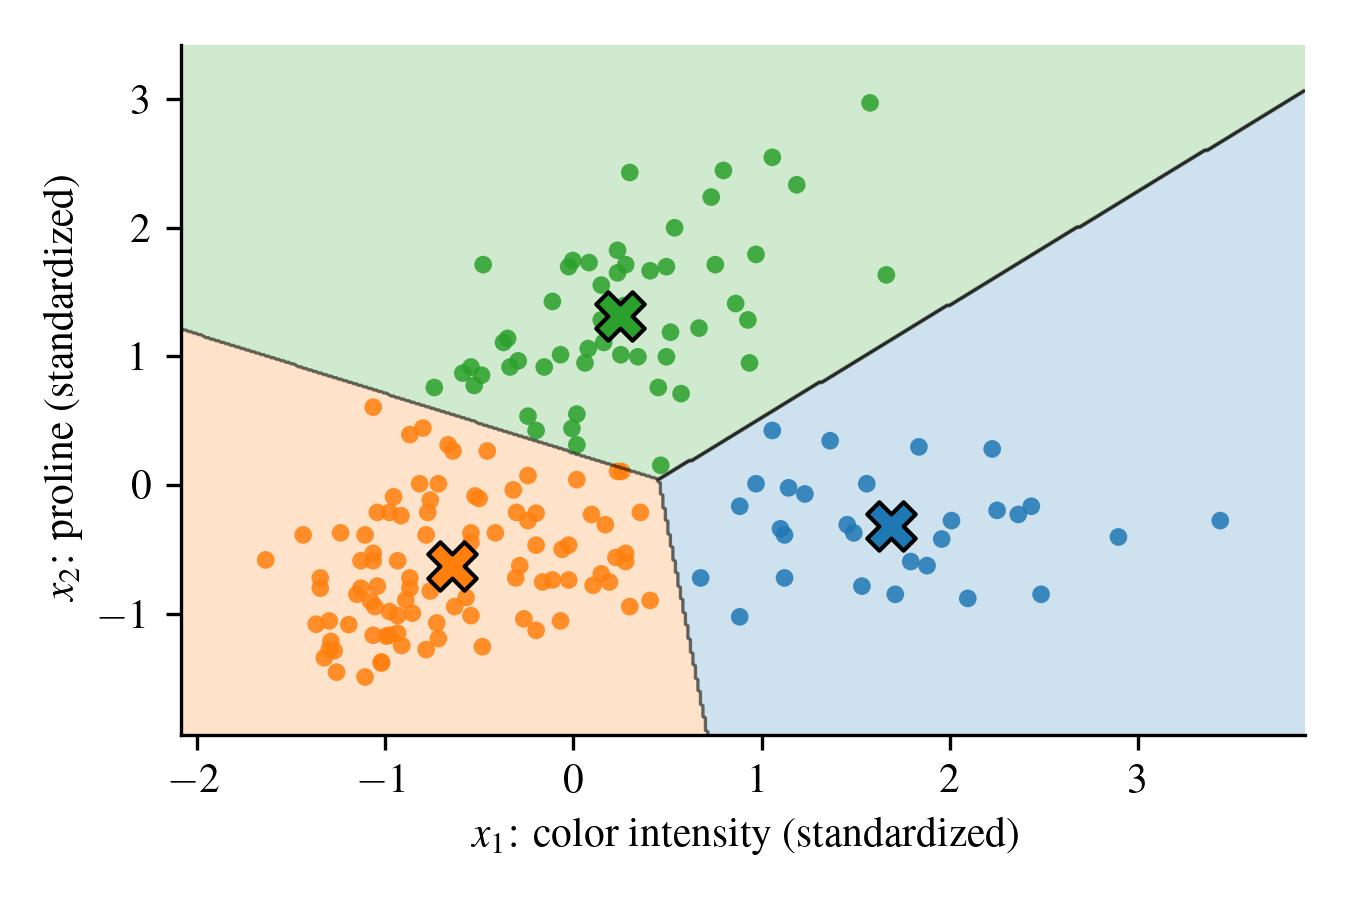
\includegraphics[width=4.5in]{../figures/K-Means_decision_regions.jpg}
	\caption{Decision regions produced by K-means after convergence. Each background color shows the region closest to one centroid, and each point is colored by its assigned K-means cluster. The large markers show the final centroid locations.}
	\label{fig:kmeans-decision-regions}
\end{figure}

Figure~\ref{fig:kmeans-centroid-updates} shows how the centroids move during the Lloyd iterations. The initial centroids are selected first, then the algorithm repeatedly assigns points and updates the centroid locations. After several iterations, the centroids settle into stable positions.

\begin{figure}[H]
	\centering
	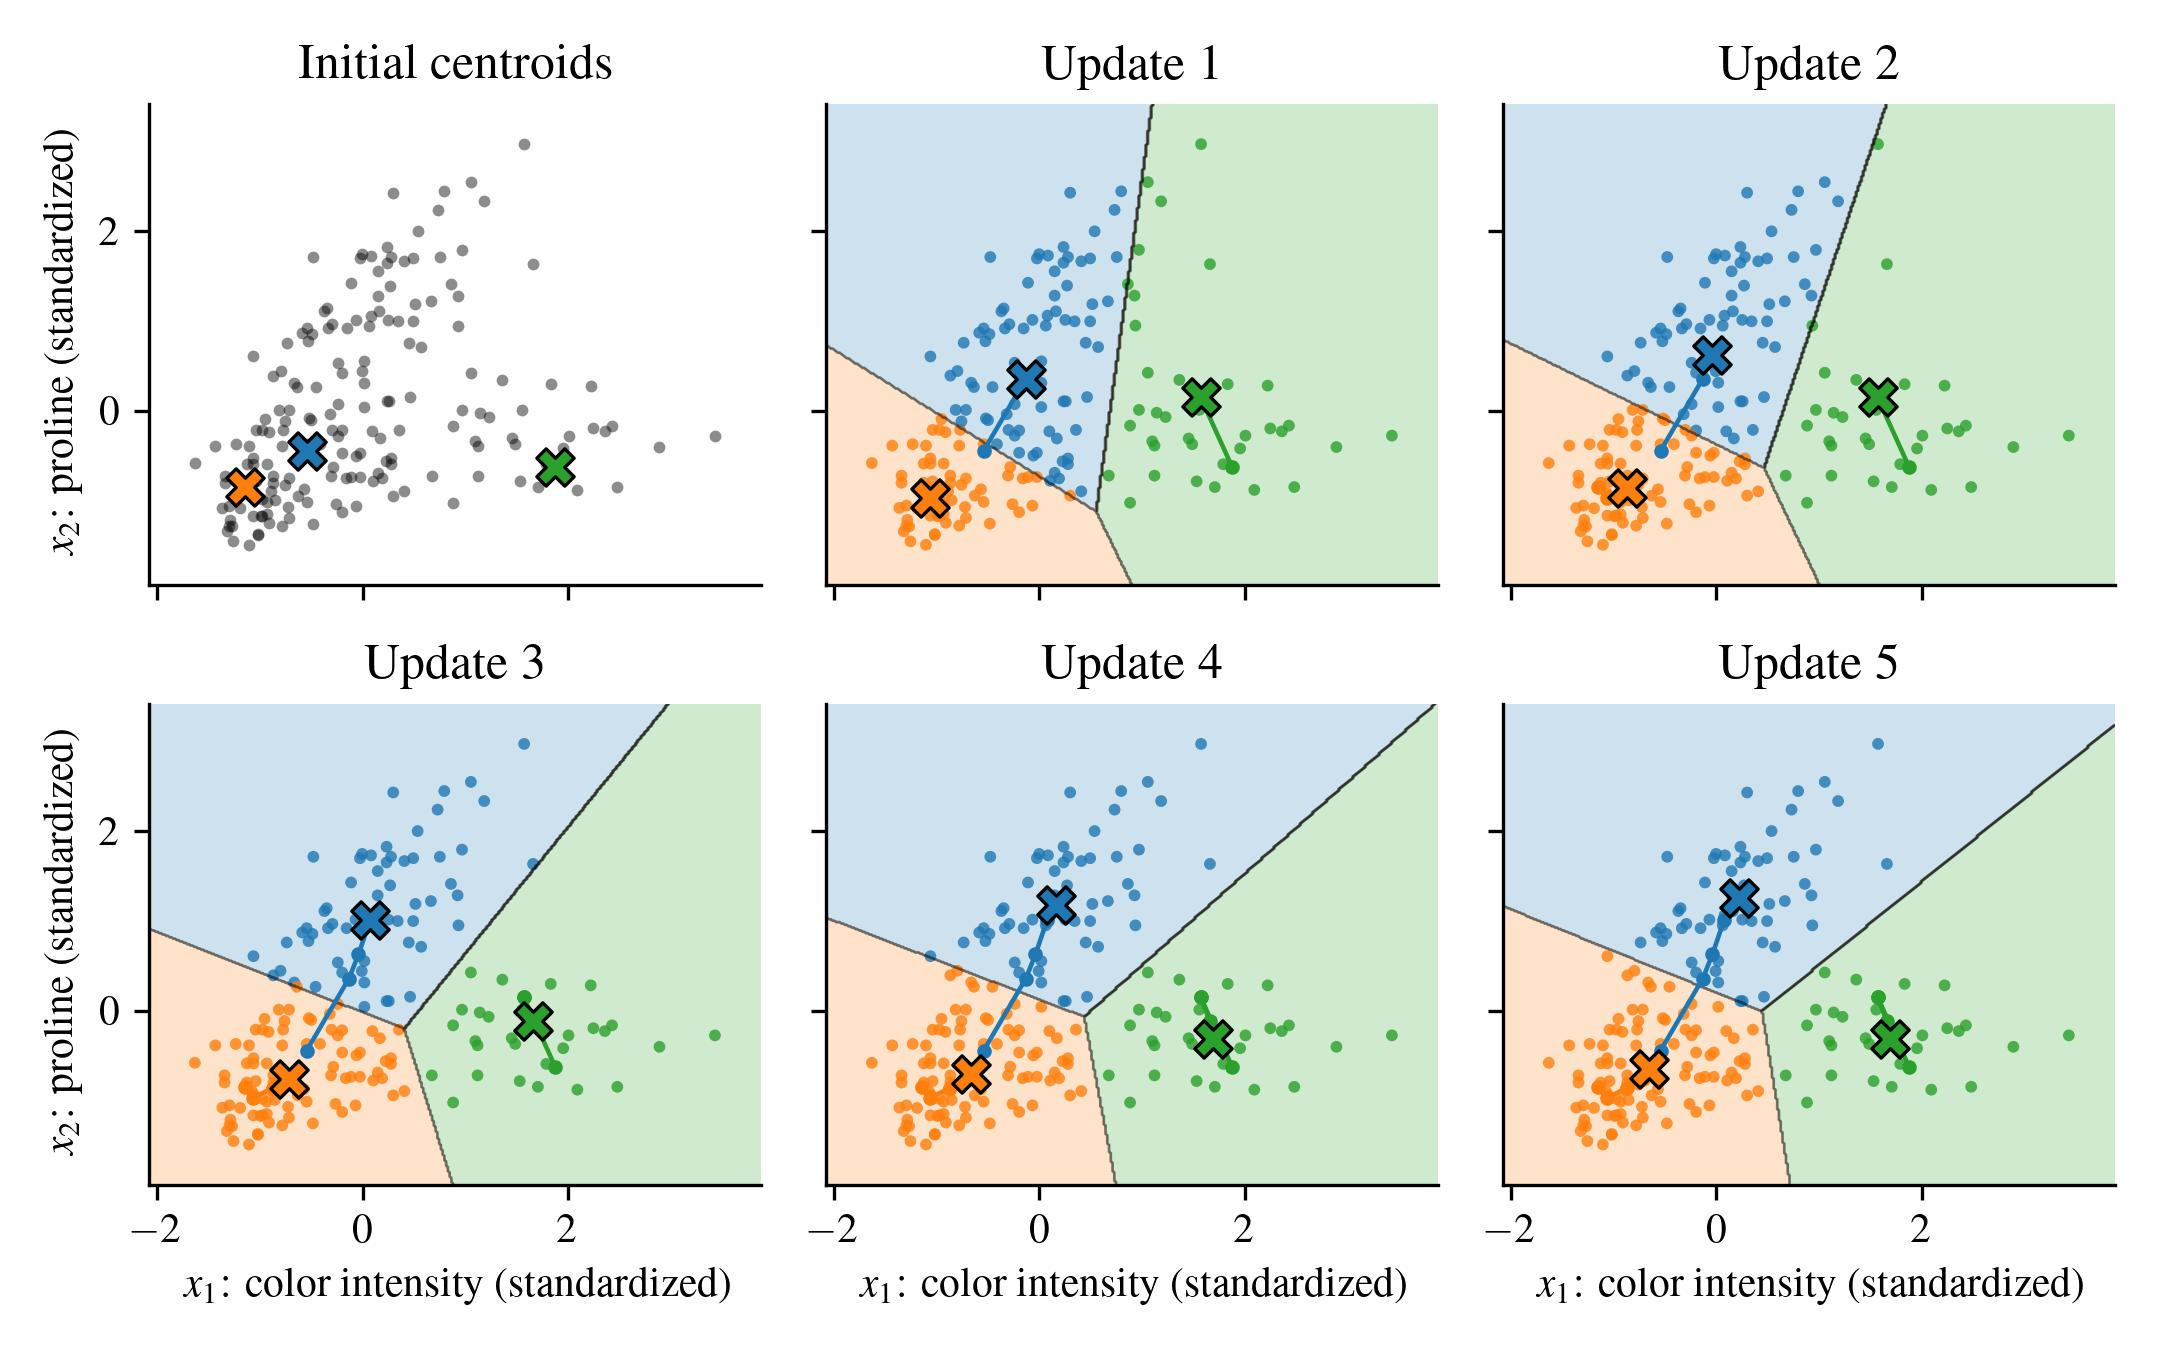
\includegraphics[width=\textwidth]{../figures/K-means_centroid_updates.jpg}
	\caption{Centroid movement during K-means. The first panel shows the initial centroids. Later panels show how the centroids move as the assignment and update steps are repeated.}
	\label{fig:kmeans-centroid-updates}
\end{figure}

Each assignment step and update step does not increase the objective function in Equation~\ref{eq:kmeans_objective}. Therefore, the algorithm eventually converges. However, the objective is not convex, so K-means is not guaranteed to find the global minimum. It can converge to different solutions depending on the initial centroid locations.

Figure~\ref{fig:kmeans-random-starts} shows this effect. Both panels use \(k=3\), but different random starts lead to different final clusterings. The lower-inertia solution has a smaller value of \(J\), meaning the points are closer to their assigned centroids on average. The higher-inertia solution is a poorer local minimum.

\begin{figure}[H]
	\centering
	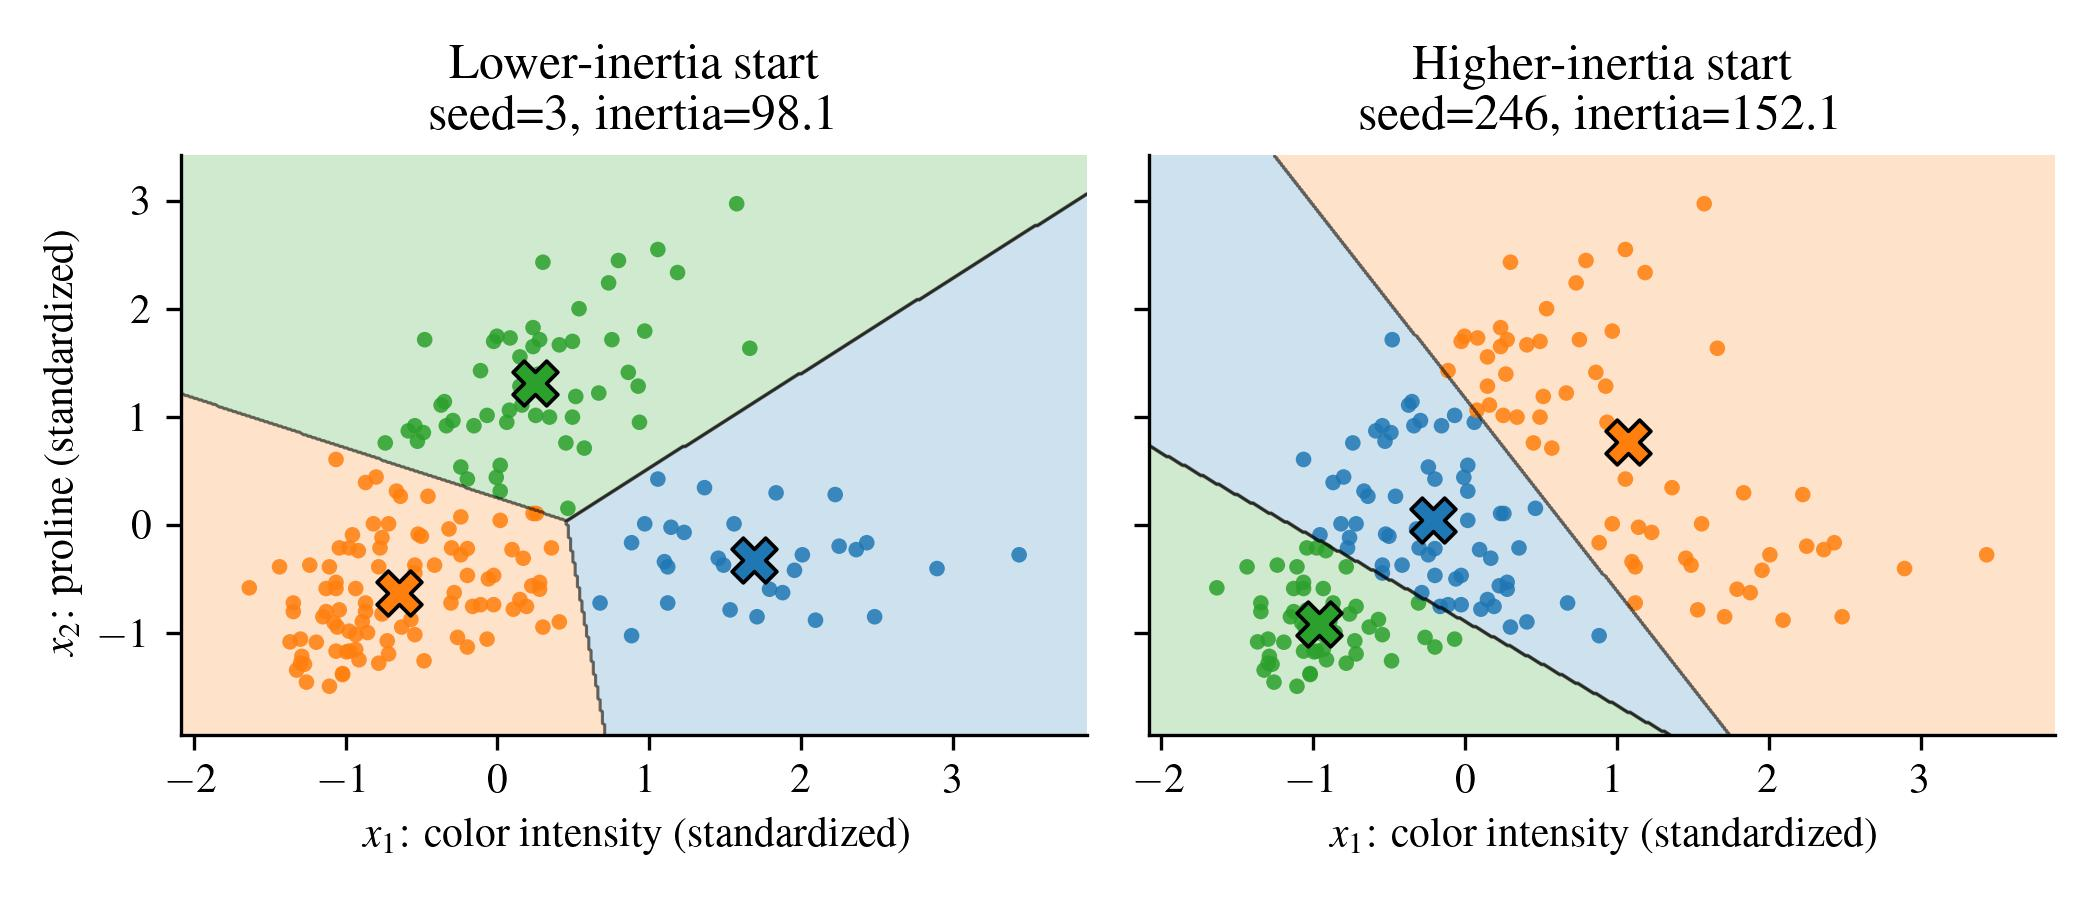
\includegraphics[width=\textwidth]{../figures/K-Means_random_starts.jpg}
	\caption{Different random initializations can lead to different K-means solutions. The lower-inertia solution is more compact, while the higher-inertia solution is a poorer local minimum.}
	\label{fig:kmeans-random-starts}
\end{figure}

A common practical fix is to run K-means multiple times with different initial centroids and keep the solution with the smallest inertia. Another common approach is to use the k-means++ initializer, which chooses more spread-out starting centroids and often improves the final result.

\subsubsection{Choosing the Number of Clusters}

The number of clusters, \(k\), must be chosen before fitting K-means. If \(k\) is too small, distinct groups may be merged together. If \(k\) is too large, one meaningful group may be split into several artificial clusters.

One common diagnostic is the elbow rule. K-means is fit for several values of \(k\), and the final inertia is plotted against \(k\). Adding more clusters almost always decreases inertia, so the goal is not simply to find the smallest value. Instead, the elbow rule looks for the value of \(k\) where the improvement begins to level off.

The decrease in inertia from adding one more cluster can be written as
\begin{equation}
    \Delta J(k)
    =
    J(k-1)-J(k).
    \label{eq:kmeans_delta_j}
\end{equation}
A large value of \(\Delta J(k)\) means that adding another cluster helped a lot. A small value means that adding another cluster gave only a small improvement.

Another useful diagnostic is the silhouette score. For point \(i\), let \(a_i\) be the average distance from point \(i\) to other points in its assigned cluster. Let \(b_i\) be the smallest average distance from point \(i\) to the points in any other cluster. The silhouette value is
\begin{equation}
    s_i
    =
    \frac{b_i-a_i}{\max(a_i,b_i)} .
    \label{eq:kmeans_silhouette}
\end{equation}

A silhouette value near \(1\) means that the point is much closer to its own cluster than to neighboring clusters. A value near \(0\) means that the point lies near a cluster boundary. A negative value suggests that the point may be assigned to the wrong cluster. The mean silhouette score over all observations can be used to compare different choices of \(k\).

\begin{figure}[H]
	\centering
	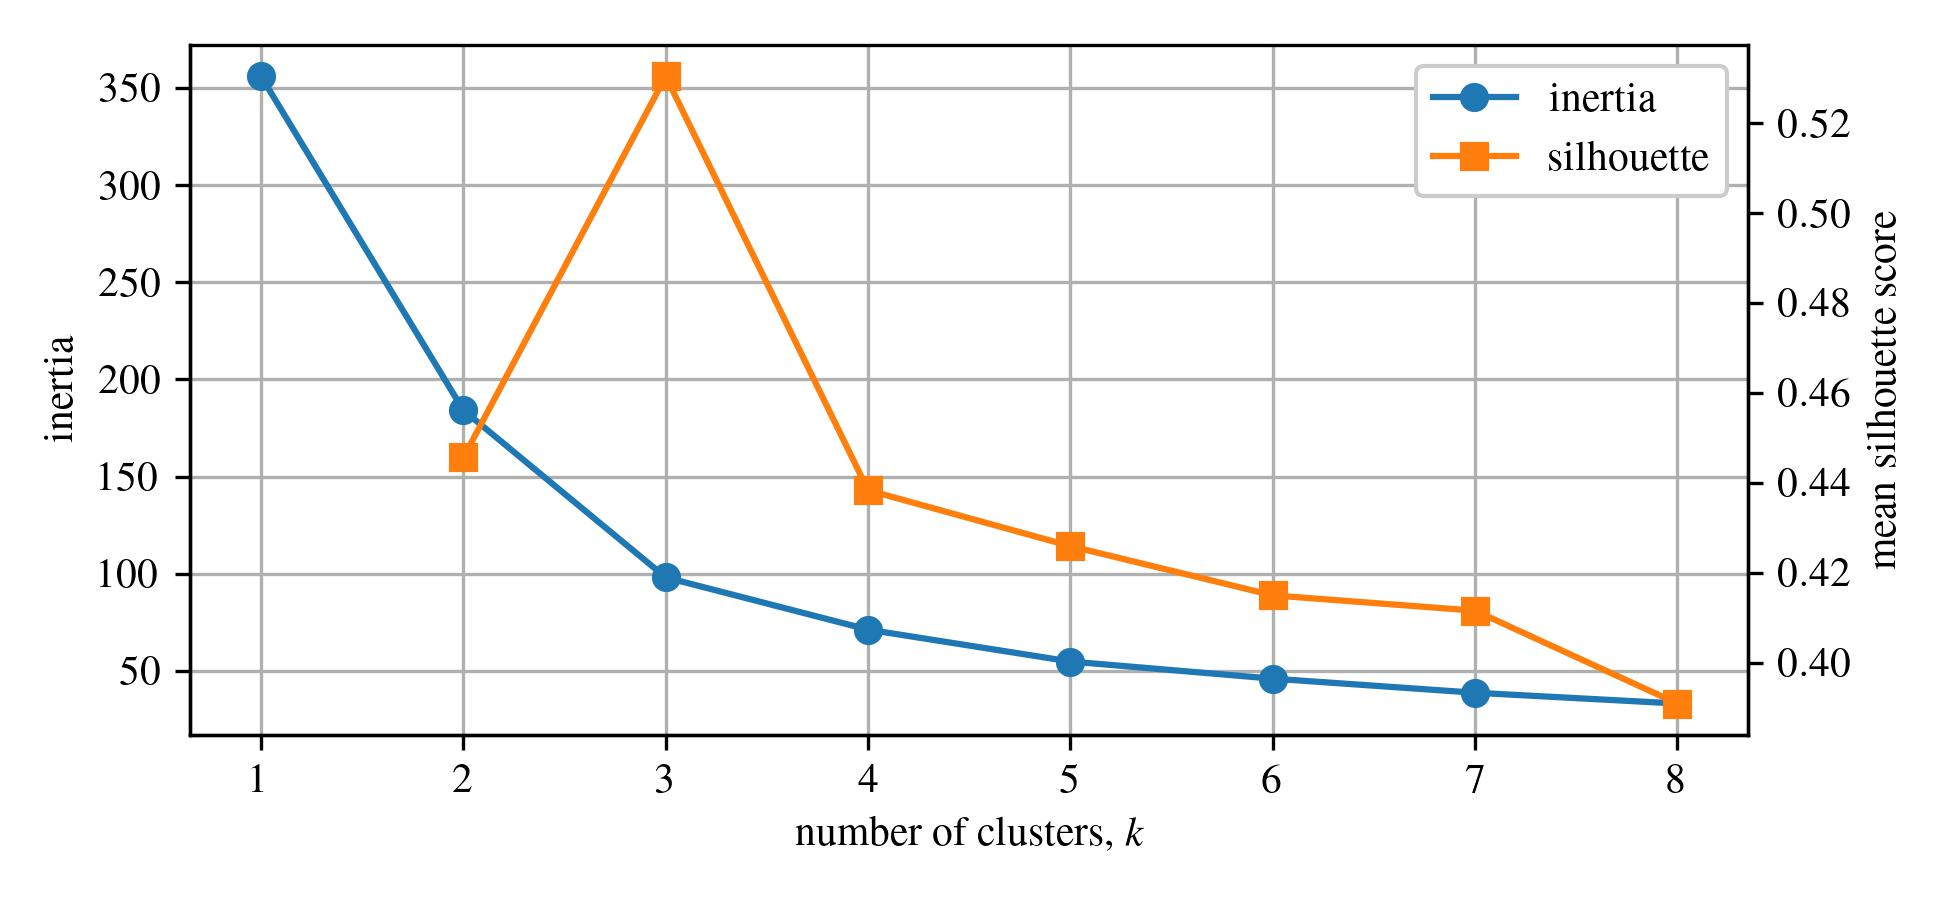
\includegraphics[width=\textwidth]{../figures/K-Means_cluster_diagnostics.jpg}
	\caption{Cluster diagnostics for the wine data. Inertia decreases as \(k\) increases, while the mean silhouette score can help identify values of \(k\) that produce well-separated clusters.}
	\label{fig:kmeans-cluster-diagnostics}
\end{figure}

For the two-dimensional wine example, the diagnostics in Figure~\ref{fig:kmeans-cluster-diagnostics} support \(k=3\). This is consistent with the three known wine classes shown in Figure~\ref{fig:kmeans-wine-data}. In real unsupervised problems, however, the true number of groups is usually not known. The final choice of \(k\) should therefore combine numerical diagnostics, visualization, and domain knowledge.

\subsubsection{Practical Notes}

K-means is usually efficient. For \(n\) observations, \(k\) clusters, and \(d\) features, one Lloyd iteration costs approximately
\begin{equation}
    O(nkd).
\end{equation}
In practice, the algorithm often converges in a small number of iterations.

Feature scaling is important. Since K-means uses Euclidean distance, a feature with a large numerical range can dominate the clustering. Standardizing continuous features before fitting K-means is often a good default choice.

Finally, K-means should be interpreted as a distance-based grouping method, not as a classifier. In the wine example, the known class labels help us judge whether the clusters make sense, but the algorithm itself does not use those labels. It simply groups points that are close together in the selected feature space.

\subsubsection{K-Means for Image Segmentation}

K-means is not limited to scatter plots or low-dimensional synthetic data. One common application is image segmentation. In this setting, each pixel is treated as an observation and the pixel values are treated as features. For a color image, each pixel may be represented by its red, green, and blue intensities,
\begin{equation}
    \mathbf{x}_i = \begin{bmatrix} R_i & G_i & B_i \end{bmatrix}^\top.
\end{equation}
K-means can then group pixels with similar colors. Replacing each pixel by its centroid color produces a compressed or segmented version of the image. This is a useful example because it shows that clustering can be used as a preprocessing step rather than as a final model.

\begin{figure}[H]
	\centering
	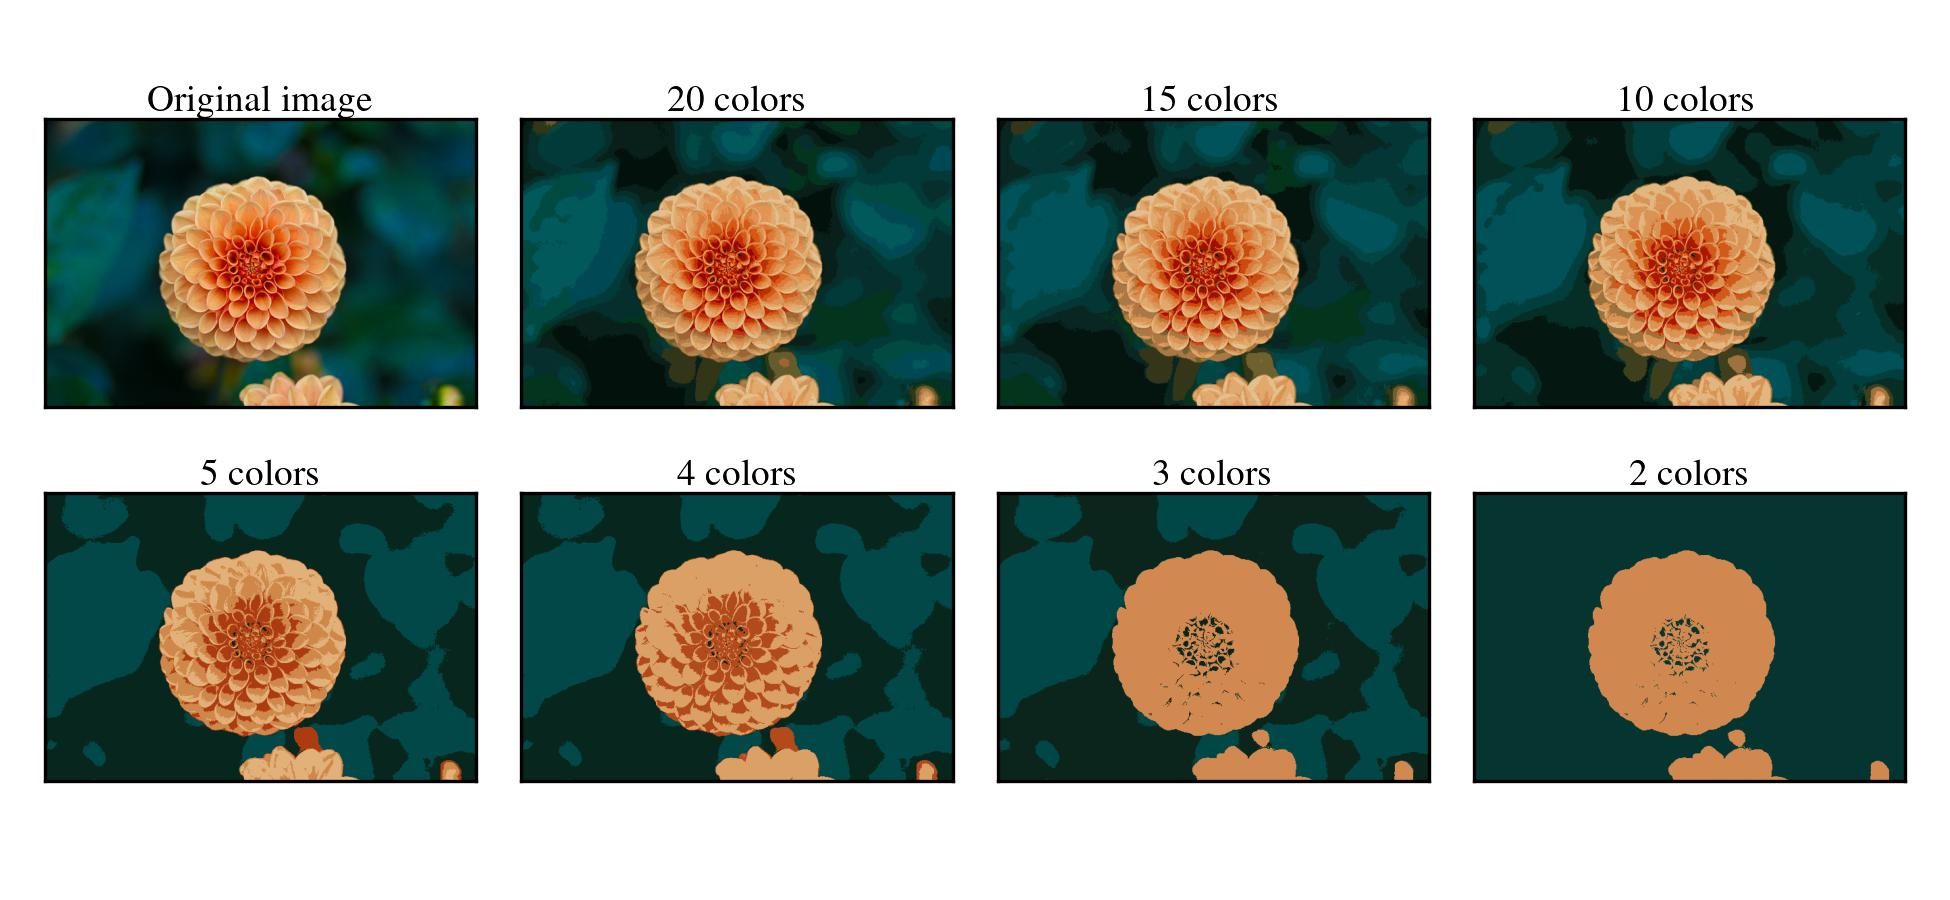
\includegraphics[width=6.5in]{../figures/K-Means_Image_segmentation}
	\caption{Image segmentation using K-means clustering, where pixels are grouped according to similarity in color space. }
	\label{fig:K-Means_Image_segmentation}
\end{figure}

\subsubsection{Limitations of K-Means}

K-means works best when clusters are compact, approximately spherical, and similar in size. It can perform poorly when clusters have irregular shapes, very different densities, or strong overlap. It is also sensitive to outliers because the centroid is a mean, and means can be pulled away from the center of a group by extreme observations.

These limitations are not necessarily failures of the algorithm. They are consequences of the model assumptions. K-means assumes that squared distance to a centroid is an appropriate measure of cluster membership. When that assumption matches the data, K-means can work very well. When the data contain curved clusters, nested clusters, or clusters with different densities, other methods may be more appropriate.

\subsection{Hierarchical Agglomerative Clustering}

Hierarchical clustering builds a nested sequence of clusters instead of returning only one fixed partition. This is useful when the number of clusters is not known in advance or when the data may contain structure at multiple levels of detail. For example, machine condition data might first divide into normal and abnormal operation, and the abnormal group might then divide into several specific fault types.



\begin{figure}[H]
	\centering
	\begin{tikzpicture}[
		wine/.style={
			draw,
			rounded corners=2pt,
			fill=red!5,
			minimum width=1.05cm,
			minimum height=0.58cm,
			align=center,
			font=\scriptsize
		},
		cluster/.style={
			draw,
			rounded corners=2pt,
			fill=orange!8,
			minimum width=2.15cm,
			minimum height=0.68cm,
			align=center,
			font=\scriptsize
		},
		profile/.style={
			draw,
			rounded corners=2pt,
			fill=yellow!10,
			minimum width=2.55cm,
			minimum height=0.72cm,
			align=center,
			font=\scriptsize
		},
		root/.style={
			draw,
			ellipse,
			fill=white,
			minimum width=3.0cm,
			minimum height=0.72cm,
			align=center,
			font=\scriptsize
		},
		branch/.style={
			black,
			line width=0.75pt,
			shorten >=2pt,
			shorten <=2pt
		}
		]
		
		% Individual wine observations
		\node[wine] (w1) at (-4.9,0.0) {Wine\\1};
		\node[wine] (w2) at (-3.5,0.0) {Wine\\2};
		\node[wine] (w3) at (-2.1,0.0) {Wine\\3};
		\node[wine] (w4) at (-0.7,0.0) {Wine\\4};
		\node[wine] (w5) at (0.7,0.0)  {Wine\\5};
		\node[wine] (w6) at (2.1,0.0)  {Wine\\6};
		\node[wine] (w7) at (3.5,0.0)  {Wine\\7};
		\node[wine] (w8) at (4.9,0.0)  {Wine\\8};
		
		% First merges: most similar pairs
		\node[cluster] (c12) at (-4.2,1.15) {low color\\low proline};
		\node[cluster] (c34) at (-1.4,1.15) {medium color\\medium proline};
		\node[cluster] (c56) at (1.4,1.15) {high color\\high proline};
		\node[cluster] (c78) at (4.2,1.15) {deep color\\lower proline};
		
		% Larger groups
		\node[profile] (c1234) at (-2.8,2.45) {lighter / medium\\wine profiles};
		\node[profile] (c5678) at (2.8,2.45) {higher-intensity\\wine profiles};
		
		% Final merge
		\node[root] (all) at (0,3.75) {all selected\\wine samples};
		
		% Branches
		\draw[branch] (w1.north) -- (c12.south);
		\draw[branch] (w2.north) -- (c12.south);
		\draw[branch] (w3.north) -- (c34.south);
		\draw[branch] (w4.north) -- (c34.south);
		\draw[branch] (w5.north) -- (c56.south);
		\draw[branch] (w6.north) -- (c56.south);
		\draw[branch] (w7.north) -- (c78.south);
		\draw[branch] (w8.north) -- (c78.south);
		
		\draw[branch] (c12.north) -- (c1234.south);
		\draw[branch] (c34.north) -- (c1234.south);
		\draw[branch] (c56.north) -- (c5678.south);
		\draw[branch] (c78.north) -- (c5678.south);
		
		\draw[branch] (c1234.north) -- (all.south);
		\draw[branch] (c5678.north) -- (all.south);
		
		% Direction cue
		\draw[-{Stealth[length=3mm]}, black, line width=0.8pt] (-5.95,0.15) -- (-5.95,3.55);
		\node[rotate=90, font=\scriptsize] at (-6.28,1.85) {bottom-up merging};
		\node[font=\scriptsize, align=center] at (0,-0.72) {Each leaf is one wine observation; nearby wines merge first.};
		
	\end{tikzpicture}
	\caption{Hierarchical agglomerative clustering using a bottom-up approach on representative wine observations. Each wine starts as its own cluster, and chemically similar wines (for example, using standardized color intensity and proline) are repeatedly merged into larger groups.}
	\label{fig:hierarchical_agglomerative_clustering}
\end{figure}





Agglomerative hierarchical clustering is a bottom-up approach. It begins by treating every observation as its own cluster. The algorithm then repeatedly merges the two closest clusters until all observations belong to a single cluster. The result is a hierarchy of possible clusterings rather than a single value of \(k\). In scikit-learn, this model is implemented by \texttt{sklearn.cluster.AgglomerativeClustering}.

The basic algorithm is:
\begin{enumerate}
    \item Start with \(n\) clusters, one for each observation.
    \item Compute the distance between every pair of clusters.
    \item Merge the two closest clusters.
    \item Update the distances between the new cluster and all remaining clusters.
    \item Repeat until all observations have been merged into one cluster.
\end{enumerate}

The key modeling decision is how to define the distance between two clusters. If \(A\) and \(B\) are two clusters, and \(d(\mathbf{x}_i,\mathbf{x}_j)\) is the distance between two observations, common linkage rules include single linkage,
\begin{equation}
    D_{\text{single}}(A,B)
    =
    \min_{\mathbf{x}_i\in A,\,\mathbf{x}_j\in B}
    d(\mathbf{x}_i,\mathbf{x}_j),
\end{equation}
complete linkage,
\begin{equation}
    D_{\text{complete}}(A,B)
    =
    \max_{\mathbf{x}_i\in A,\,\mathbf{x}_j\in B}
    d(\mathbf{x}_i,\mathbf{x}_j),
\end{equation}
and average linkage,
\begin{equation}
    D_{\text{average}}(A,B)
    =
    \frac{1}{|A||B|}
    \sum_{\mathbf{x}_i\in A}\sum_{\mathbf{x}_j\in B}
    d(\mathbf{x}_i,\mathbf{x}_j).
\end{equation}

Single linkage compares the closest points in two clusters. This can capture long, chain-like clusters, but it can also connect groups through a small number of bridging points. Complete linkage compares the farthest points in two clusters, which tends to produce compact groups. Average linkage is a compromise because it uses all pairwise distances between the two clusters.

Ward linkage uses a different idea. Instead of directly measuring pairwise distances between clusters, Ward linkage merges the two clusters that lead to the smallest increase in within-cluster variation. If \(C\) is a cluster with centroid \(\boldsymbol{\mu}_C\), its within-cluster sum of squares is
\begin{equation}
    W(C)=\sum_{\mathbf{x}_i\in C}\left\lVert \mathbf{x}_i-\boldsymbol{\mu}_C\right\rVert^2.
\end{equation}
When clusters \(A\) and \(B\) are merged, Ward linkage considers the increase
\begin{equation}
    \Delta W = W(A\cup B)-W(A)-W(B).
\end{equation}
This makes Ward linkage conceptually similar to K-means because both methods favor compact clusters with small within-cluster variation.

\subsubsection{Dendrograms}

A dendrogram is a tree diagram that shows the order in which clusters are merged. At the bottom of the dendrogram, each observation begins as its own cluster. As the height increases, clusters merge together. The height at which two branches merge represents the dissimilarity between those clusters. Cutting the dendrogram at a chosen height produces a particular clustering solution.

The advantage of a dendrogram is that it lets the user inspect the clustering structure before committing to a specific number of clusters. Large vertical gaps in the dendrogram suggest that clusters were merged only after a large increase in dissimilarity. Cutting through one of these gaps often gives a reasonable partition of the data.

Hierarchical clustering is especially useful for exploratory analysis and visualization. However, it can be computationally expensive for large data sets because many pairwise distances must be stored or updated. As with K-means, feature scaling is usually important because the distance metric determines which observations appear close together.
\subsection{Density-Based Methods (DBSCAN and HDBSCAN)}

Density-based clustering methods define clusters as dense regions of the feature space separated by sparse regions. This is a different assumption from K-means. K-means represents each cluster by a centroid and assigns each observation to the nearest centroid. DBSCAN, by contrast, does not begin with a centroid. Instead, it asks whether a point has enough nearby neighbors to be considered part of a dense region.

Figure~\ref{fig:DBSCAN_vs_make_moons} illustrates why this difference matters. The top row uses the \texttt{make\_moons} dataset, and the bottom row uses the \texttt{make\_circles} dataset. Both examples contain non-spherical clusters. K-means struggles because the clusters are curved, so assigning points to the nearest center cuts across the natural geometry of the data. DBSCAN performs better because it follows connected regions of high point density.

\begin{figure}[H]
	\centering
	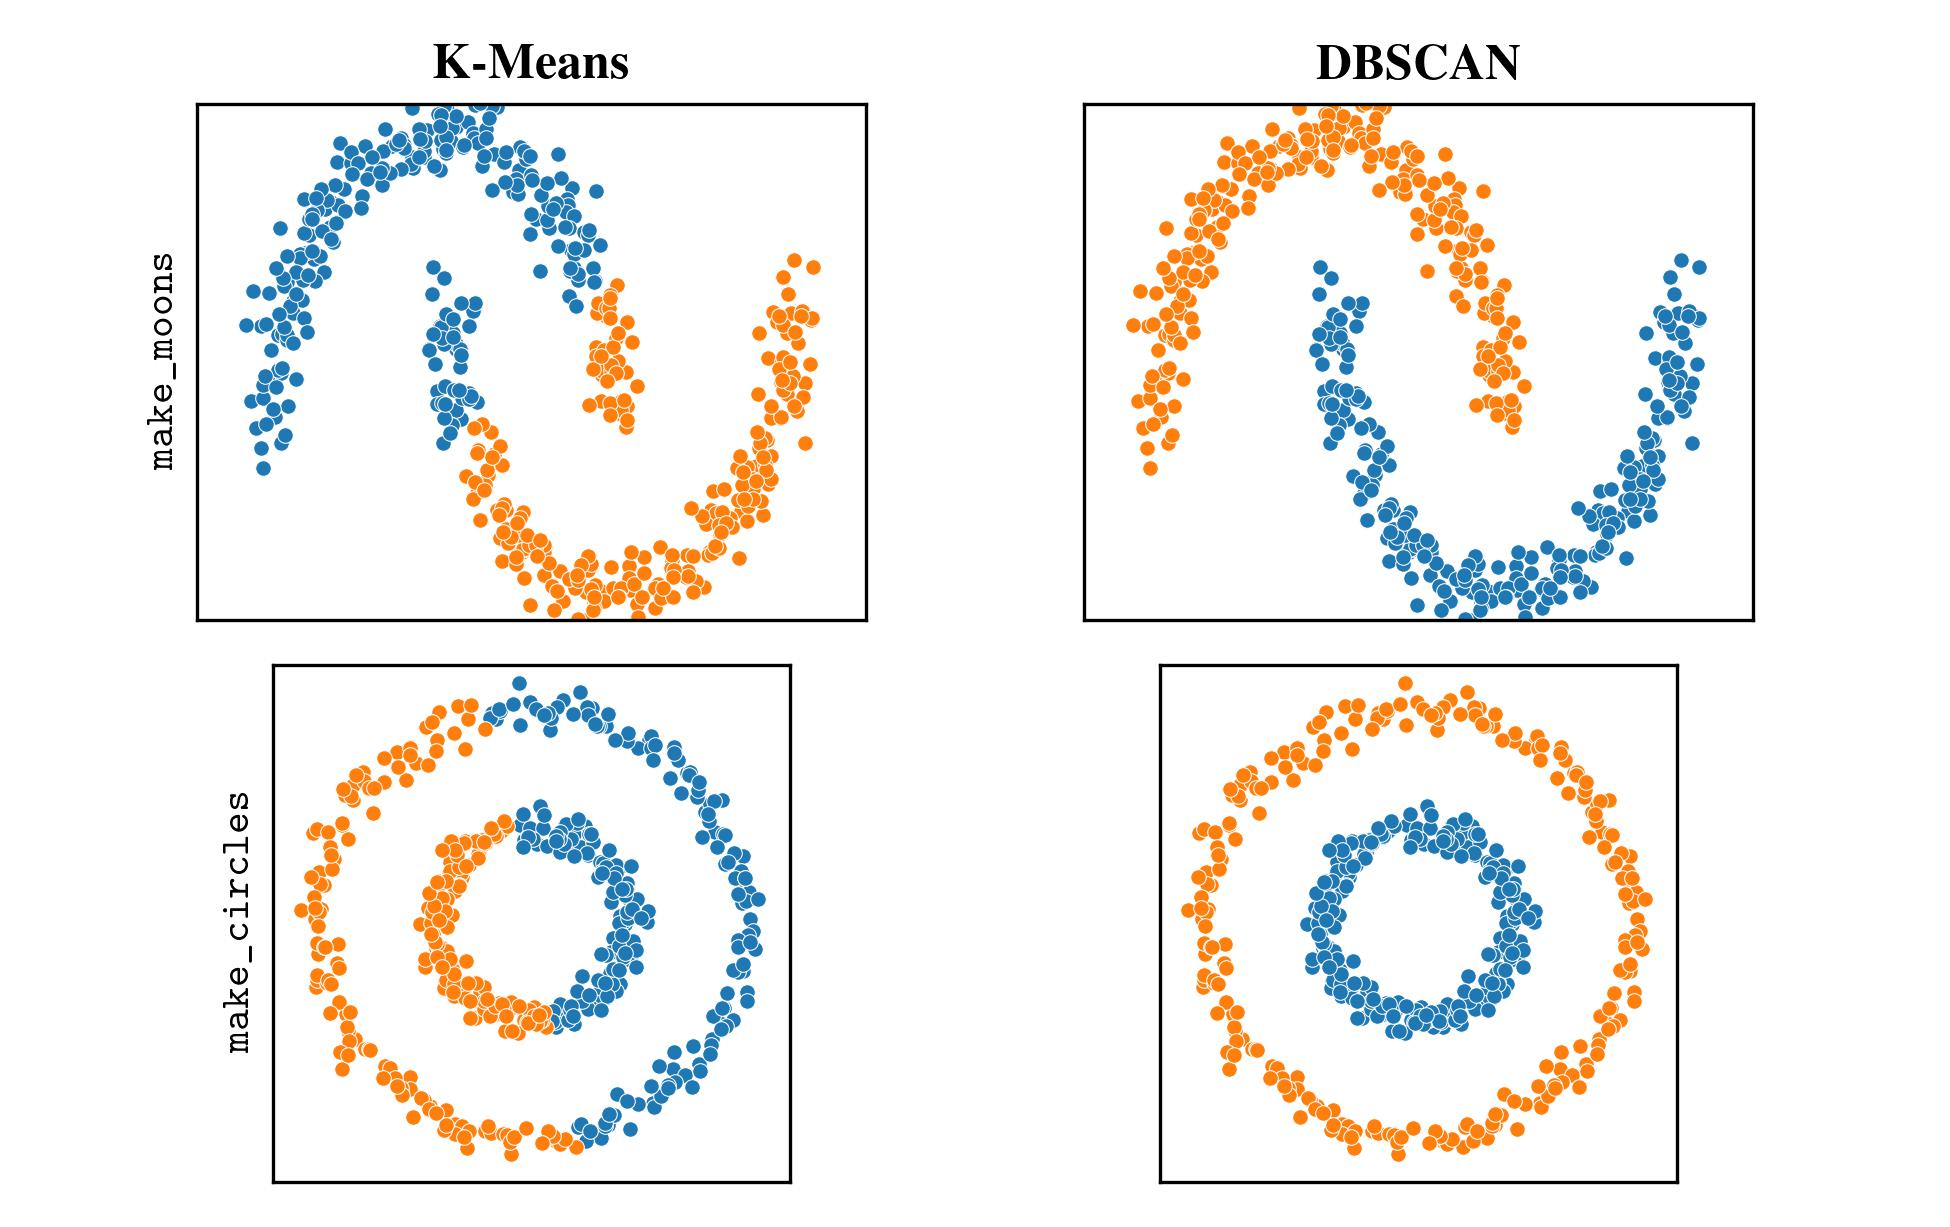
\includegraphics[width=6.5in]{../figures/DBSCAN_vs_k-means}
	\caption{Comparison of K-means and DBSCAN on non-spherical data. K-means assigns observations to the nearest centroid, while DBSCAN groups connected dense regions.}
	\label{fig:DBSCAN_vs_make_moons}
\end{figure}

DBSCAN stands for Density-Based Spatial Clustering of Applications with Noise. In scikit-learn, it is implemented by \texttt{sklearn.cluster.DBSCAN}. The method has two main parameters:
\begin{itemize}
    \item \(\epsilon\), which defines the radius of a local neighborhood.
    \item \(\mathrm{minPts}\), called \texttt{min\_samples} in scikit-learn, which defines how many points must be nearby for a region to be considered dense.
\end{itemize}

For a point \(\mathbf{x}_i\), the \(\epsilon\)-neighborhood is the set of all points within distance \(\epsilon\):
\begin{equation}
    N_\epsilon(\mathbf{x}_i)
    =
    \left\{
    \mathbf{x}_j \in X :
    d(\mathbf{x}_i,\mathbf{x}_j) \leq \epsilon
    \right\}.
\end{equation}
Here \(d(\mathbf{x}_i,\mathbf{x}_j)\) is usually Euclidean distance. A point is called a core point if its neighborhood contains at least \(\mathrm{minPts}\) points:
\begin{equation}
    \left|N_\epsilon(\mathbf{x}_i)\right|
    \geq
    \mathrm{minPts}.
\end{equation}

This definition is the main idea behind DBSCAN. A core point sits in a dense part of the data. A border point is not dense enough to be a core point, but it lies close to a core point. A noise point is neither a core point nor close enough to a core point to be attached to a cluster.

DBSCAN builds clusters by connecting core points. If two core points are within distance \(\epsilon\), they are part of the same dense region. If a chain of core points connects one part of the data to another, all of those points are assigned to the same cluster. Border points are then attached to nearby clusters, while noise points remain unassigned.

The choice of \(\epsilon\) is important. Figure~\ref{fig:DBSCAN_eps_too_small} shows what happens when \(\epsilon\) is too small. The neighborhoods are so small that most points do not have enough neighbors to become core points. As a result, DBSCAN labels most of the data as noise. This does not mean the data have no structure; it means the density scale chosen by \(\epsilon\) is too small for this dataset.

\begin{figure}[H]
	\centering
	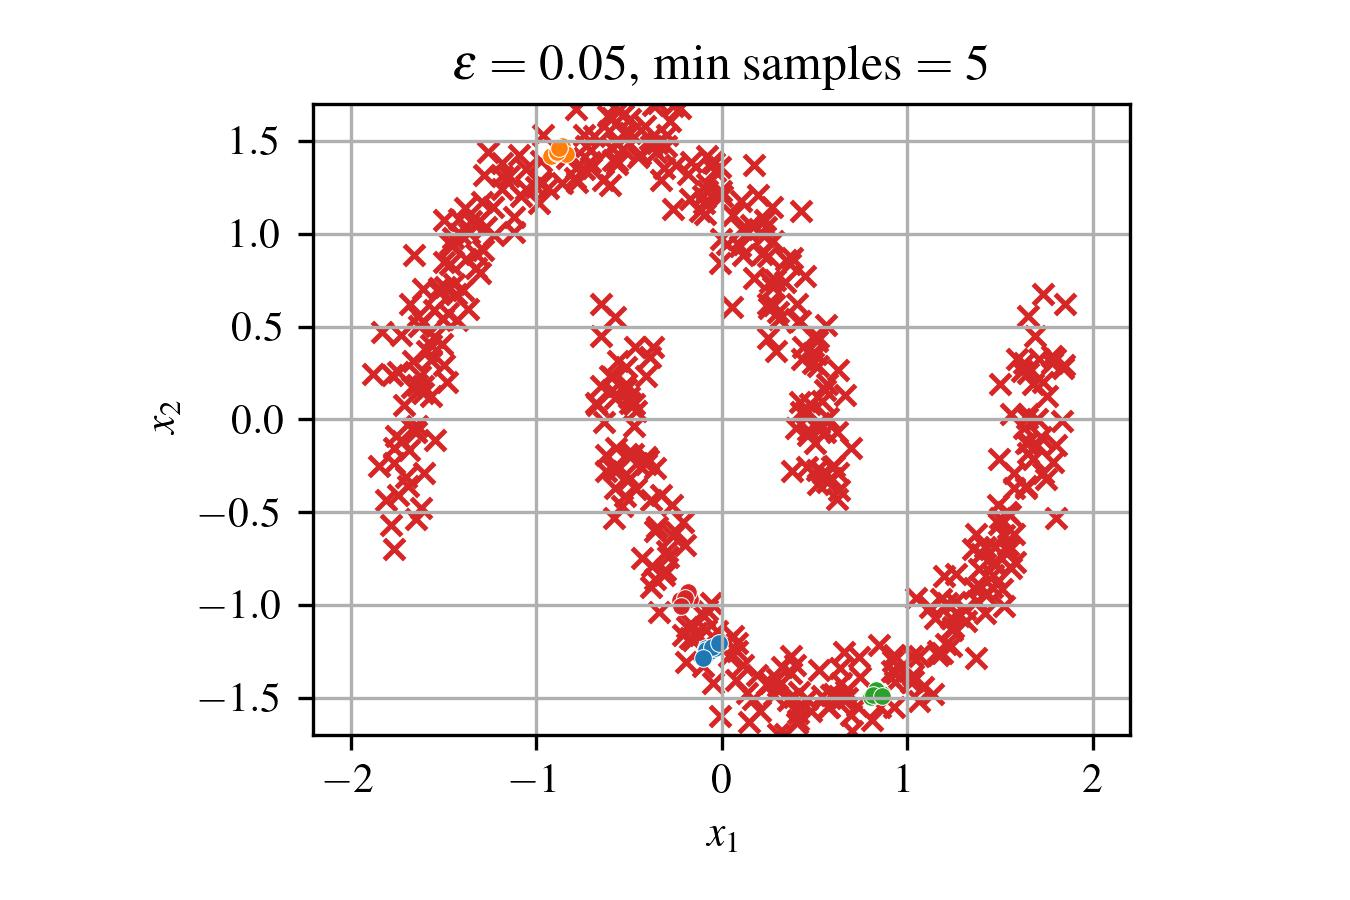
\includegraphics[width=4.75in]{../figures/DBSCAN_eps_too_small}
	\caption{DBSCAN with \(\epsilon\) too small. Most observations are labeled as noise because each point has too few neighbors inside its local neighborhood.}
	\label{fig:DBSCAN_eps_too_small}
\end{figure}

Figure~\ref{fig:DBSCAN_eps_neighborhoods} shows a more useful value of \(\epsilon\). The transparent circles represent local \(\epsilon\)-neighborhoods around core points. These neighborhoods overlap along each moon-shaped region, allowing DBSCAN to connect the points into two clusters. A few isolated observations remain labeled as noise because they do not belong to any dense region.

\begin{figure}[H]
	\centering
	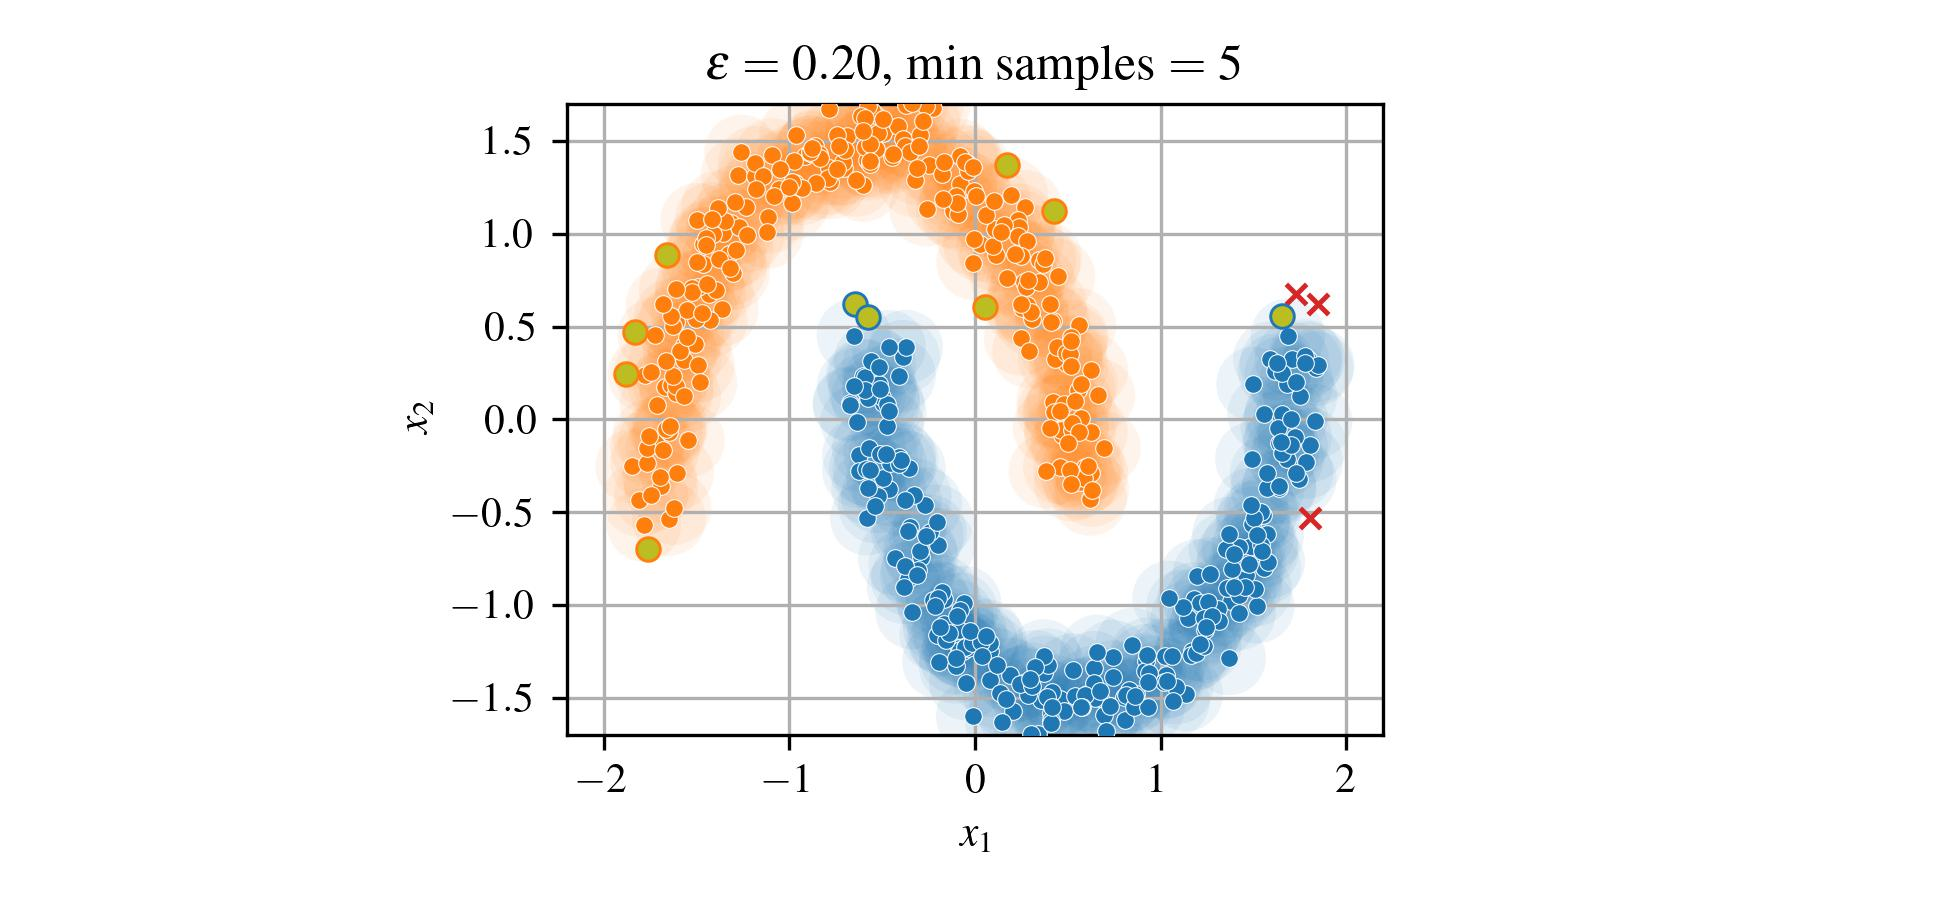
\includegraphics[width=4.75in]{../figures/DBSCAN_eps_neighborhoods}
	\caption{DBSCAN with a larger \(\epsilon\), where overlapping neighborhoods connect core points into two curved clusters. Points that do not belong to a dense region are labeled as noise.}
	\label{fig:DBSCAN_eps_neighborhoods}
\end{figure}

The three figures together show the basic DBSCAN story. K-means is a centroid-based method, so it works best when clusters can be described by their centers. DBSCAN is a density-based method, so it works best when clusters can be described as connected dense regions. This makes DBSCAN useful for curved clusters, irregular shapes, and datasets that contain outliers.

However, DBSCAN is sensitive to the value of \(\epsilon\). If \(\epsilon\) is too small, many points are labeled as noise. If \(\epsilon\) is too large, separate clusters may be merged together. The parameter \(\mathrm{minPts}\) also matters. Larger values of \(\mathrm{minPts}\) require denser neighborhoods and can make the method more conservative. Smaller values allow clusters to form more easily but may also make the model more sensitive to noise.

A common way to choose \(\epsilon\) is to use a nearest-neighbor distance plot. For each observation, compute the distance to its \(k\)-th nearest neighbor, where \(k\) is usually chosen to match \(\mathrm{minPts}\). These distances are sorted from smallest to largest. A sharp bend in the curve suggests a transition between dense regions and sparse regions, and this bend can be used as a starting value for \(\epsilon\).

HDBSCAN extends DBSCAN by reducing the need to choose one fixed value of \(\epsilon\). Instead of clustering the data at a single neighborhood radius, HDBSCAN builds a hierarchy of density-based clusterings over many density levels. Clusters that remain stable over a range of density levels are kept, while unstable clusters are discarded. This makes HDBSCAN useful when different clusters have different densities.

One way to understand HDBSCAN is through the core distance. Let \(d_c(\mathbf{x}_i)\) be the distance from \(\mathbf{x}_i\) to its \(\mathrm{minPts}\)-th nearest neighbor. Points in dense regions have small core distances, while points in sparse regions have large core distances. HDBSCAN uses this idea to make sparse points appear farther apart and dense points appear more strongly connected.

A common distance used in HDBSCAN is the mutual reachability distance:
\begin{equation}
    d_m(\mathbf{x}_i,\mathbf{x}_j)
    =
    \max
    \left\{
    d_c(\mathbf{x}_i),
    d_c(\mathbf{x}_j),
    d(\mathbf{x}_i,\mathbf{x}_j)
    \right\}.
\end{equation}
This distance increases the separation between sparse points while preserving connections inside dense regions. The algorithm then builds a hierarchy from this density-adjusted distance structure.

\subsubsection{When to Use Density-Based Clustering}

Density-based clustering is a good choice when the clusters may have irregular shapes or when the data contain outliers. It is often useful for spatial data, sensor data, and operating-regime discovery. For example, a machine may spend most of its time in several dense regions corresponding to common operating states, while unusual transients or faults may appear as sparse points between those regions.

DBSCAN is usually easiest to explain and visualize because its two parameters have a direct interpretation: \(\epsilon\) sets the neighborhood size, and \(\mathrm{minPts}\) sets how dense a neighborhood must be. HDBSCAN is often more flexible in practice because it can handle clusters with different densities. In both cases, the result still depends on the feature representation and distance metric, so feature scaling should usually be applied before fitting the model.


\subsection{Gaussian Mixture Models}

\begin{figure}[H]
	\centering
	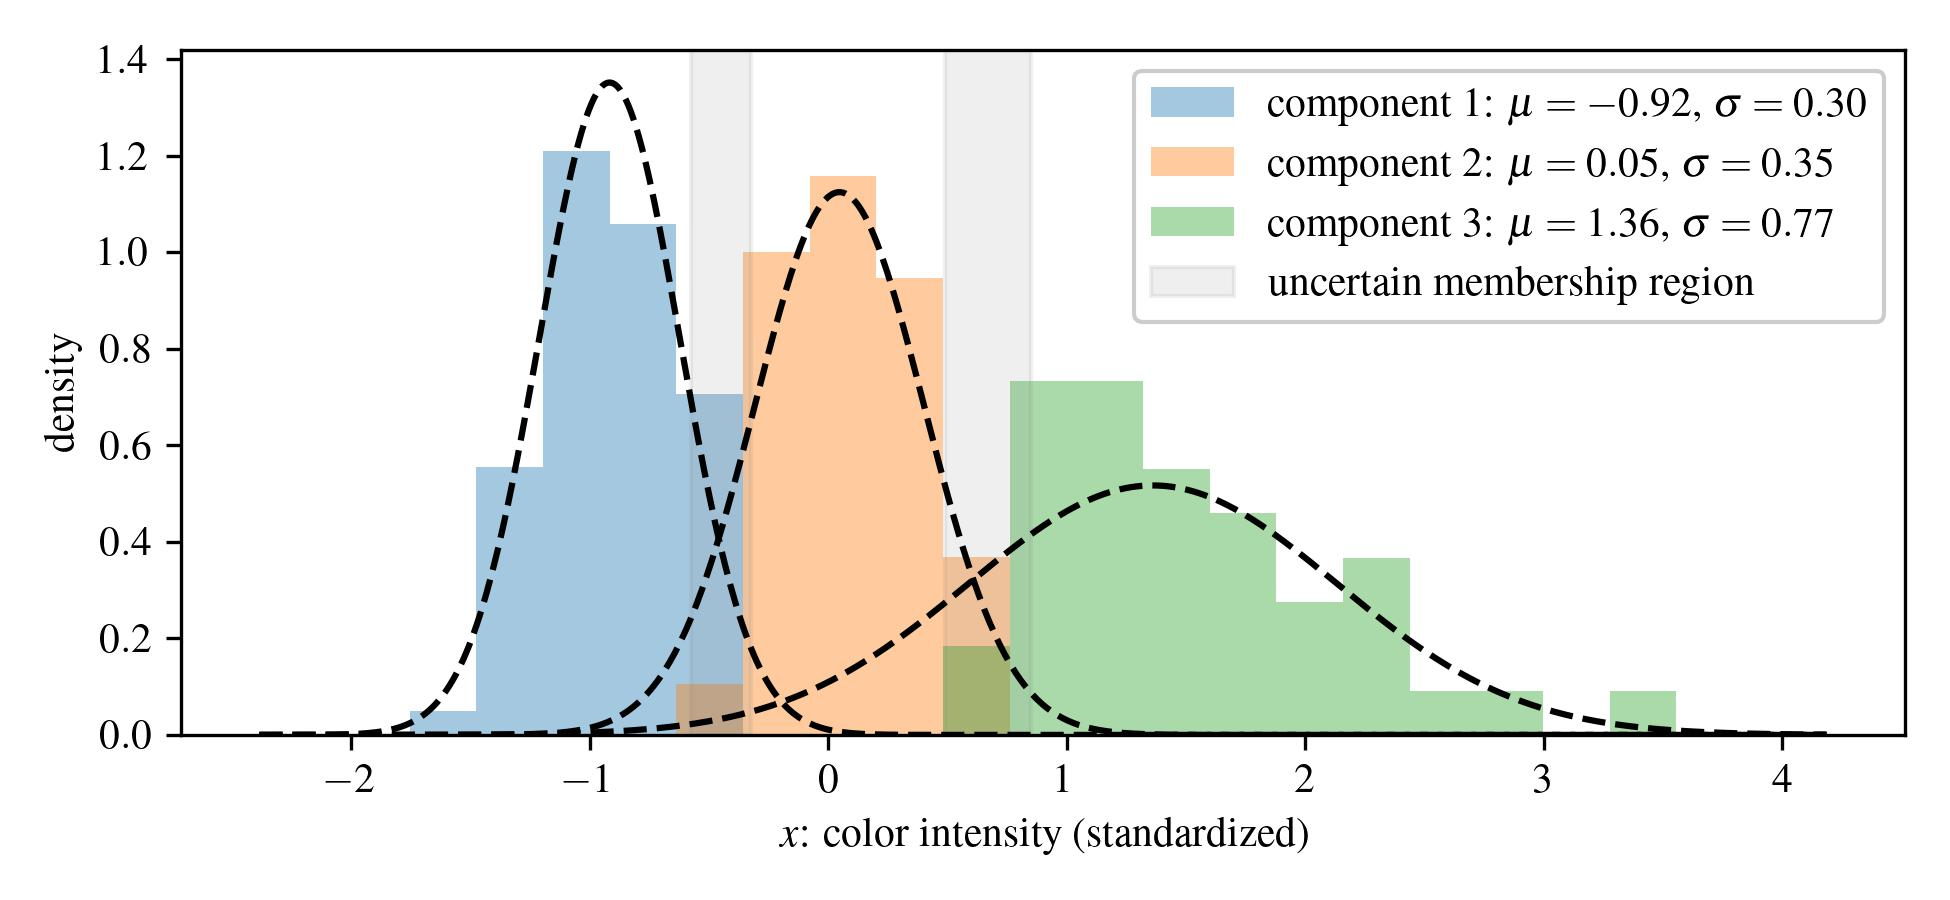
\includegraphics[width=6.5in]{../figures/Gaussian_general_idea}
	\caption{General idea of Gaussian mixture modeling applied to the wine data using standardized color intensity. The histograms show wine observations grouped by their most likely Gaussian component, the dashed curves show the fitted component densities, and the shaded regions indicate feature values where component membership is uncertain.}
	\label{fig:Gaussian_general_idea}
\end{figure}

K-means assigns each observation to exactly one cluster. Gaussian mixture models provide a probabilistic alternative. Figure~\ref{fig:Gaussian_general_idea} shows the general idea using the wine data: instead of placing each wine only into a single centroid-based group, the model represents the data as a weighted combination of Gaussian components. Each component has its own mean and spread, shown by the dashed Gaussian curves in the figure.

This probabilistic view is useful when groups overlap. A wine observation near the overlap between two components may not clearly belong to only one group. Instead, the model can assign probabilities that describe how strongly the observation belongs to each component. More generally, each Gaussian component has its own mean and covariance matrix, which allows clusters to have different shapes, orientations, and sizes.

A Gaussian mixture model with \(k\) components has probability density
\begin{equation}
    p(\mathbf{x})
    =
    \sum_{j=1}^{k}
    \pi_j
    \mathcal{N}
    \left(
        \mathbf{x}
        \mid
        \boldsymbol{\mu}_j,
        \boldsymbol{\Sigma}_j
    \right),
    \label{eq:gmm_density}
\end{equation}
where \(\pi_j\) is the mixing weight for component \(j\), \(\boldsymbol{\mu}_j\) is the component mean, and \(\boldsymbol{\Sigma}_j\) is the component covariance matrix. The mixing weights satisfy
\begin{equation}
    \pi_j \geq 0,
    \qquad
    \sum_{j=1}^{k}\pi_j=1.
\end{equation}
The multivariate Gaussian density is
\begin{equation}
    \mathcal{N}
    \left(
        \mathbf{x}
        \mid
        \boldsymbol{\mu},
        \boldsymbol{\Sigma}
    \right)
    =
    \frac{1}
    {(2\pi)^{d/2}|\boldsymbol{\Sigma}|^{1/2}}
    \exp
    \left[
        -\frac{1}{2}
        (\mathbf{x}-\boldsymbol{\mu})^\top
        \boldsymbol{\Sigma}^{-1}
        (\mathbf{x}-\boldsymbol{\mu})
    \right].
\end{equation}

The mean \(\boldsymbol{\mu}\) controls the center of the Gaussian component, while the covariance matrix \(\boldsymbol{\Sigma}\) controls its spread, shape, and orientation. This makes Gaussian mixture models more flexible than K-means. K-means effectively represents each cluster with only a center, while a Gaussian mixture model represents each component with both a center and a covariance structure.

In scikit-learn, Gaussian mixture models are implemented by \texttt{sklearn.mixture.GaussianMixture}. The fitted model can be used to predict cluster labels, estimate probabilities of component membership, sample new observations, or evaluate the likelihood of new data.

\begin{figure}[H]
	\centering
	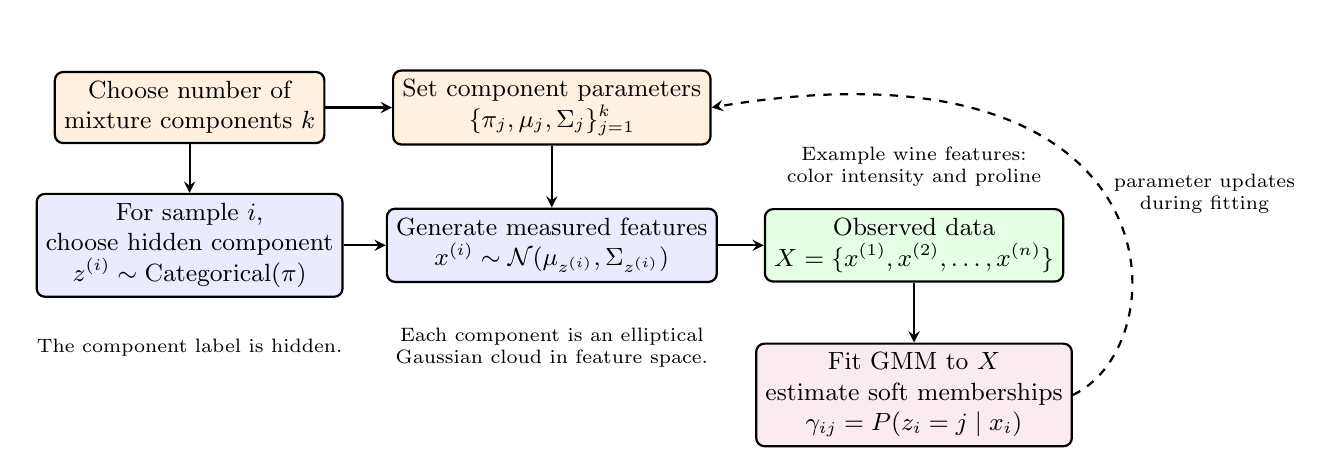
\begin{tikzpicture}[
		>=stealth,
		thick,
		process/.style={
			rectangle,
			draw,
			rounded corners=3pt,
			minimum width=3.35cm,
			minimum height=0.9cm,
			align=center,
			fill=blue!8
		},
		param/.style={
			rectangle,
			draw,
			rounded corners=3pt,
			minimum width=3.35cm,
			minimum height=0.9cm,
			align=center,
			fill=orange!12
		},
		data/.style={
			rectangle,
			draw,
			rounded corners=3pt,
			minimum width=3.35cm,
			minimum height=0.9cm,
			align=center,
			fill=green!10
		},
		output/.style={
			rectangle,
			draw,
			rounded corners=3pt,
			minimum width=3.35cm,
			minimum height=0.9cm,
			align=center,
			fill=purple!8
		},
		note/.style={
			align=center,
			font=\scriptsize
		},
		every node/.style={font=\small}
		]
		
		% ------------------------------------------------------------
		% Top row: model setup and parameters
		% ------------------------------------------------------------
		\node[param] (k) at (-4.6,2.0)
		{Choose number of\\mixture components \(k\)};
		
		\node[param] (params) at (0,2.0)
		{Set component parameters\\
			\(\{\pi_j,\mu_j,\Sigma_j\}_{j=1}^{k}\)};
		
		% ------------------------------------------------------------
		% Middle row: generative process
		% ------------------------------------------------------------
		\node[process] (latent) at (-4.6,0.25)
		{For sample \(i\),\\
			choose hidden component\\
			\(z^{(i)} \sim \mathrm{Categorical}(\pi)\)};
		
		\node[process] (sample) at (0,0.25)
		{Generate measured features\\
			\(x^{(i)} \sim
			\mathcal{N}\!\left(\mu_{z^{(i)}},\Sigma_{z^{(i)}}\right)\)};
		
		\node[data] (observed) at (4.6,0.25)
		{Observed data\\
			\(X=\{x^{(1)},x^{(2)},\ldots,x^{(n)}\}\)};
		
		% ------------------------------------------------------------
		% Bottom row: fitted-model interpretation
		% ------------------------------------------------------------
		\node[output] (fit) at (4.6,-1.65)
		{Fit GMM to \(X\)\\
			estimate soft memberships\\
			\(\gamma_{ij}=P(z_i=j \mid x_i)\)};
		
		% ------------------------------------------------------------
		% Main flow arrows
		% ------------------------------------------------------------
		\draw[->] (k) -- (params);
		\draw[->] (k) -- (latent);
		\draw[->] (params) -- (sample);
		\draw[->] (latent) -- (sample);
		\draw[->] (sample) -- (observed);
		\draw[->] (observed) -- (fit);
		
		% ------------------------------------------------------------
		% Dashed feedback arrow routed outside the chart
		% ------------------------------------------------------------
		\draw[->, dashed]
		(fit.east)
		.. controls (8,-1) and (8,3)
		.. (params.east)
		node[pos=0.52, right, note] {parameter updates\\during fitting};
		
		% ------------------------------------------------------------
		% Explanatory notes
		% ------------------------------------------------------------
		\node[note] at (-4.6,-1.05)
		{The component label is hidden.};
		
		\node[note] at (0,-1.05)
		{Each component is an elliptical\\Gaussian cloud in feature space.};
		
		\node[note] at (4.6,1.25)
		{Example wine features:\\color intensity and proline};
		
	\end{tikzpicture}
	
	\caption{Flow-chart representation of a Gaussian mixture model for the wine data. The model assumes that each wine is associated with an unobserved mixture component, and then its measured feature vector is generated from the Gaussian distribution for that component. When the model is fit to data, it estimates soft component probabilities rather than only hard cluster labels.}
	\label{fig:Gaussian_mixture_model}
\end{figure}


\subsubsection{Soft Cluster Assignments}

A major difference between K-means and Gaussian mixture models is that Gaussian mixtures produce soft assignments. Instead of assigning observation \(\mathbf{x}_i\) only to the nearest component, the model estimates the probability that \(\mathbf{x}_i\) belongs to each component. This probability is called the responsibility of component \(j\) for observation \(i\):
\begin{equation}
    \gamma_{ij}
    =
    P(z_i=j\mid \mathbf{x}_i)
    =
    \frac{
        \pi_j
        \mathcal{N}
        \left(
            \mathbf{x}_i
            \mid
            \boldsymbol{\mu}_j,
            \boldsymbol{\Sigma}_j
        \right)
    }
    {
        \sum_{\ell=1}^{k}
        \pi_\ell
        \mathcal{N}
        \left(
            \mathbf{x}_i
            \mid
            \boldsymbol{\mu}_\ell,
            \boldsymbol{\Sigma}_\ell
        \right)
    }.
    \label{eq:gmm_responsibility}
\end{equation}
Here \(z_i\) is a latent variable indicating which component generated observation \(i\). The responsibilities satisfy
\begin{equation}
    0\leq \gamma_{ij}\leq 1,
    \qquad
    \sum_{j=1}^{k}\gamma_{ij}=1.
\end{equation}
A hard cluster label can still be produced by assigning each observation to the component with the largest responsibility:
\begin{equation}
    \hat{z}_i = \arg\max_j \gamma_{ij}.
\end{equation}

Figure~\ref{fig:Gaussian_mixture_cluster} shows a Gaussian mixture model fit to the wine data using standardized color intensity and proline as the two features. The contours show the fitted mixture density, the dashed curves show the decision regions between mixture components, and the colored points show the component assignments.

\begin{figure}[H]
	\centering
	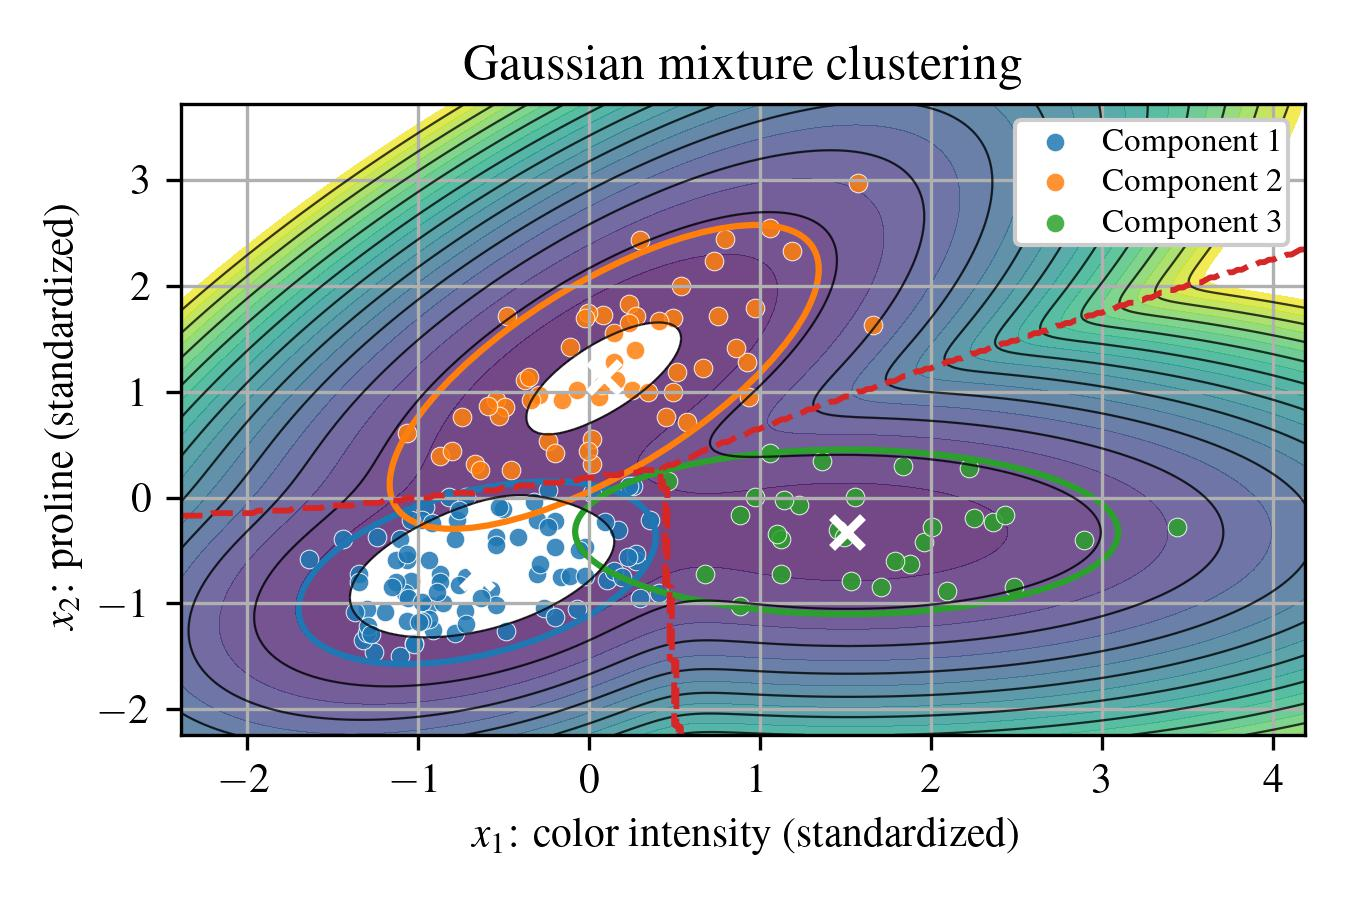
\includegraphics[width=4.5in]{../figures/Gaussian_mixture_cluster}
	\caption{Gaussian mixture clustering applied to the wine data using standardized color intensity and proline. Each observation is assigned to the component with the largest posterior probability.}
	\label{fig:Gaussian_mixture_cluster}
\end{figure}

Soft assignments are useful when clusters overlap. An observation near the boundary between two groups may receive probabilities such as \(0.55\) and \(0.45\), indicating uncertainty. This is often more informative than a hard label alone, especially when the data contain partially overlapping groups.

\subsubsection{Expectation-Maximization}

The parameters of a Gaussian mixture model are usually estimated with the expectation-maximization algorithm, abbreviated EM. The objective is to maximize the log-likelihood of the observed data:
\begin{equation}
    \ell(\Theta)
    =
    \sum_{i=1}^{n}
    \log
    \left[
        \sum_{j=1}^{k}
        \pi_j
        \mathcal{N}
        \left(
            \mathbf{x}_i
            \mid
            \boldsymbol{\mu}_j,
            \boldsymbol{\Sigma}_j
        \right)
    \right],
\end{equation}
where
\begin{equation}
    \Theta
    =
    \left\{
        \pi_j,
        \boldsymbol{\mu}_j,
        \boldsymbol{\Sigma}_j
    \right\}_{j=1}^{k}
\end{equation}
denotes all mixture parameters. Directly maximizing this expression is difficult because the component identity \(z_i\) is unknown. EM handles this by alternating between estimating the hidden component memberships and updating the model parameters.

In the expectation step, the responsibilities \(\gamma_{ij}\) are computed using Equation~\ref{eq:gmm_responsibility}. In the maximization step, the parameters are updated using weighted averages. Let
\begin{equation}
    N_j=\sum_{i=1}^{n}\gamma_{ij}
\end{equation}
be the effective number of observations assigned to component \(j\). The updates are
\begin{equation}
    \pi_j = \frac{N_j}{n},
\end{equation}
\begin{equation}
    \boldsymbol{\mu}_j
    =
    \frac{1}{N_j}
    \sum_{i=1}^{n}
    \gamma_{ij}\mathbf{x}_i,
\end{equation}
and
\begin{equation}
    \boldsymbol{\Sigma}_j
    =
    \frac{1}{N_j}
    \sum_{i=1}^{n}
    \gamma_{ij}
    \left(\mathbf{x}_i-\boldsymbol{\mu}_j\right)
    \left(\mathbf{x}_i-\boldsymbol{\mu}_j\right)^\top.
\end{equation}
These two steps are repeated until the log-likelihood changes very little between iterations.

\subsubsection{Covariance Structure}

The covariance matrix controls the shape and orientation of each Gaussian component. This gives Gaussian mixtures more flexibility than K-means. A spherical covariance produces circular clusters in two dimensions. A diagonal covariance allows each feature direction to have a different variance but does not rotate the cluster. A tied covariance uses the same covariance matrix for every component. A full covariance matrix allows each component to have its own tilted ellipse and can capture correlation between features.

Figure~\ref{fig:Gaussian_mixture_model_covariance} compares two covariance assumptions on the wine data. With a tied covariance, all components share the same covariance matrix, so the ellipses have the same shape and orientation. With a spherical covariance, each component is forced to be circular in the standardized feature space. These constraints can make the model easier to estimate, but they may also prevent the model from matching the shape of the data.

\begin{figure}[H]
	\centering
	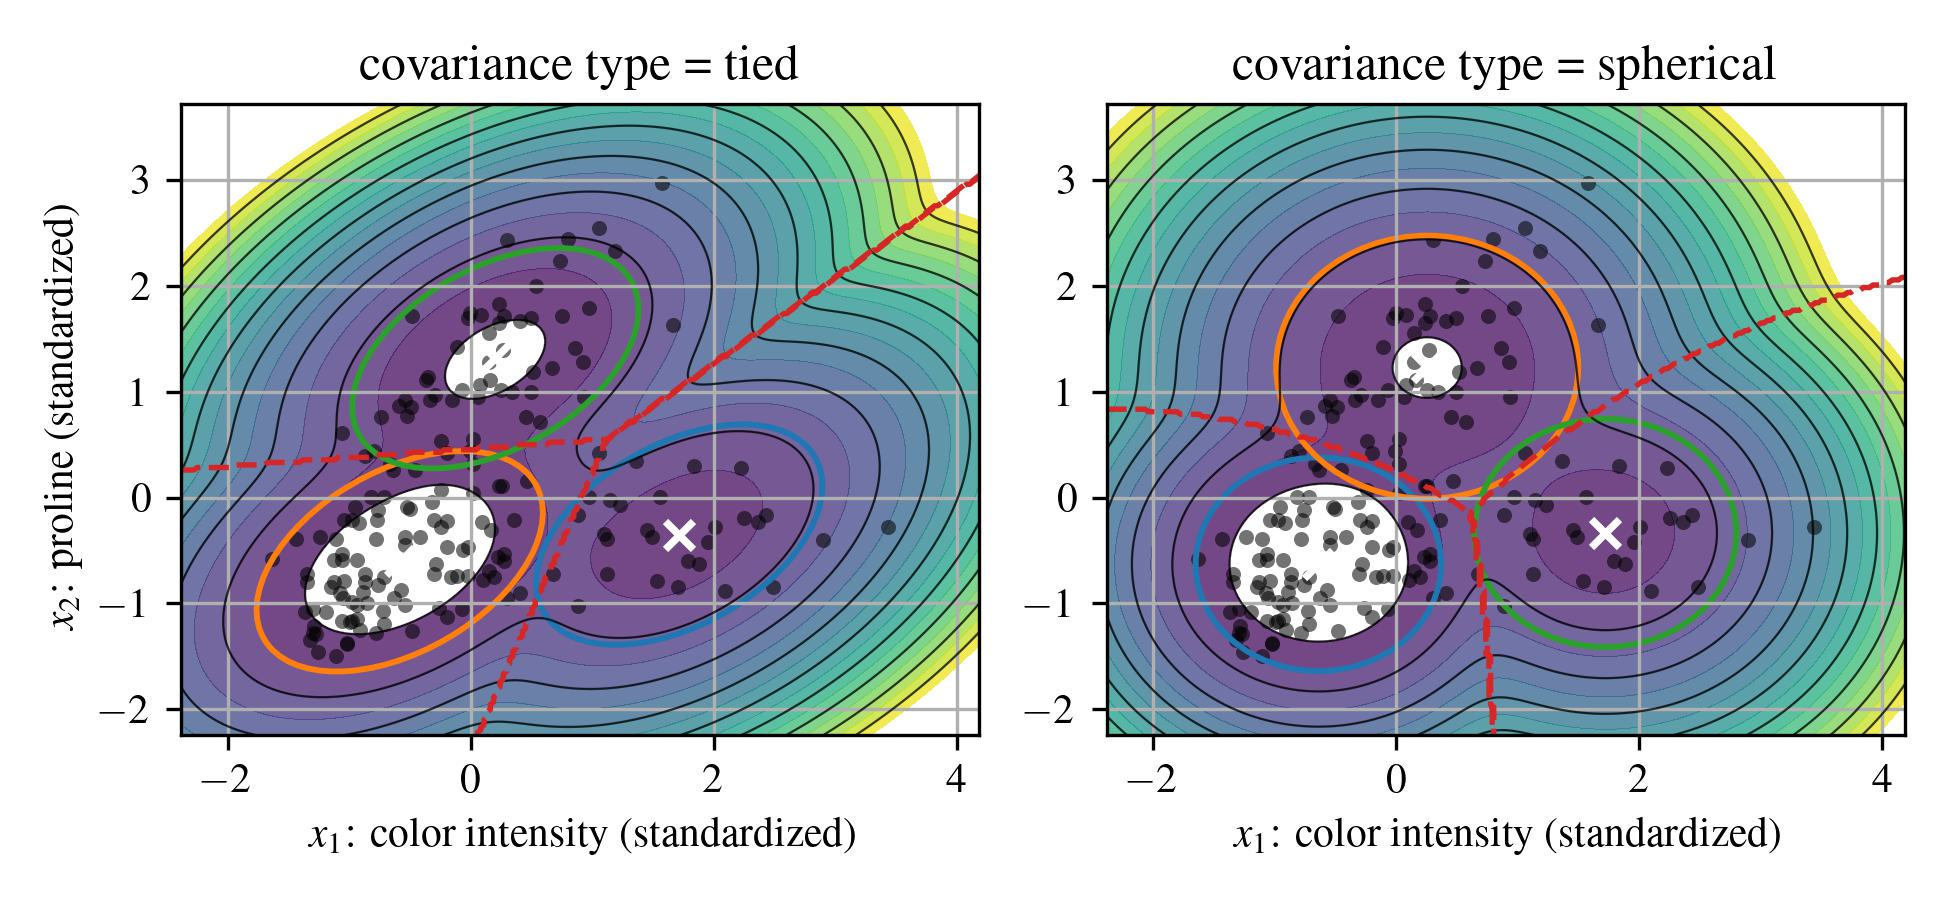
\includegraphics[width=6.5in]{../figures/Gaussian_mixture_covariance}
	\caption{Effect of covariance structure on Gaussian mixture components fit to the wine data. The tied model shares one covariance matrix across all components, while the spherical model restricts each component to have circular contours in the standardized feature space.}
	\label{fig:Gaussian_mixture_model_covariance}
\end{figure}

The covariance choice is important because it controls model flexibility. A full covariance model can fit complex elliptical clusters, but it has more parameters and can overfit small data sets. A spherical or diagonal covariance model is more restrictive, but it may be more stable when the number of observations is limited.

Gaussian mixture models also require choosing the number of components, \(k\). The elbow rule can be used, but likelihood-based criteria are common because GMMs are probabilistic models. Two common choices are the Akaike information criterion (AIC) and Bayesian information criterion (BIC):
\begin{equation}
    \mathrm{AIC}
    =
    2p - 2\ell(\hat{\Theta}),
\end{equation}
\begin{equation}
    \mathrm{BIC}
    =
    p\log(n) - 2\ell(\hat{\Theta}),
\end{equation}
where \(p\) is the number of estimated parameters and \(\ell(\hat{\Theta})\) is the maximized log-likelihood. Lower values indicate a better tradeoff between model fit and model complexity. BIC penalizes model complexity more strongly than AIC when \(n\) is large.

\subsubsection{Relationship Between K-Means and Gaussian Mixtures}

K-means can be viewed as a limiting case of a Gaussian mixture model. If all mixture components have spherical covariance matrices with the same small variance, then assigning a point to the component with the largest probability becomes similar to assigning it to the nearest mean. In that sense, K-means is like a hard-assignment, equal-variance version of a Gaussian mixture model.

This connection is useful because it explains the behavior of both methods. K-means is simpler and often faster, but it cannot represent uncertainty in cluster membership. Gaussian mixtures are more flexible and probabilistic, but they require estimating more parameters and can be sensitive to initialization, covariance assumptions, and the number of components.

\subsection{Anomaly Detection}

Clustering methods are often used not only to find groups, but also to identify observations that do not fit any group well. These unusual observations are called anomalies, outliers, or novelties depending on the application. In engineering, anomalies may correspond to faulty sensors, rare operating conditions, damaged components, unusual loading events, or data-entry errors.

A simple anomaly detection idea is to fit a model to the normal data and then flag observations that have low likelihood under that model. For a single Gaussian distribution, the density of an observation is
\begin{equation}
    p(\mathbf{x})
    =
    \mathcal{N}
    \left(
        \mathbf{x}
        \mid
        \boldsymbol{\mu},
        \boldsymbol{\Sigma}
    \right).
\end{equation}
An anomaly can be defined by applying a threshold \(\tau\):
\begin{equation}
    \hat{y}(\mathbf{x})
    =
    \begin{cases}
    \text{anomaly}, & p(\mathbf{x}) < \tau,\\
    \text{normal}, & p(\mathbf{x}) \geq \tau.
    \end{cases}
\end{equation}
Equivalently, since log-likelihoods are easier to compute numerically, the threshold can be applied to the log-likelihood:
\begin{equation}
    \log p(\mathbf{x}) < \log \tau.
\end{equation}

For a Gaussian model, anomaly detection is closely related to the Mahalanobis distance,
\begin{equation}
    D_M(\mathbf{x})
    =
    \sqrt{
        (\mathbf{x}-\boldsymbol{\mu})^\top
        \boldsymbol{\Sigma}^{-1}
        (\mathbf{x}-\boldsymbol{\mu})
    }.
\end{equation}
This distance measures how far \(\mathbf{x}\) is from the mean after accounting for the covariance of the data. A point may look far away in Euclidean distance but not be unusual if it lies along a high-variance direction. Conversely, a point may have moderate Euclidean distance but be highly unusual if it lies along a low-variance direction.

Gaussian mixture models extend this idea to data with multiple normal operating regimes. Instead of using one Gaussian density, the mixture density from Equation~\ref{eq:gmm_density} is used. An observation is considered normal if it has high likelihood under at least one component and anomalous if it has low likelihood under the entire mixture. This is useful when a system has several legitimate operating states. A point may be far from one operating state but close to another, so a single Gaussian model may be too restrictive.

Figure~\ref{fig:Gaussian_anomaly_detection} shows this idea using the wine data. The Gaussian mixture model is fit to the standardized color intensity and proline features. Observations with low likelihood under the fitted mixture are marked as potential anomalies. These points are not necessarily ``bad'' measurements; they are simply observations that the fitted model considers unusual relative to the rest of the data.

\begin{figure}[H]
	\centering
	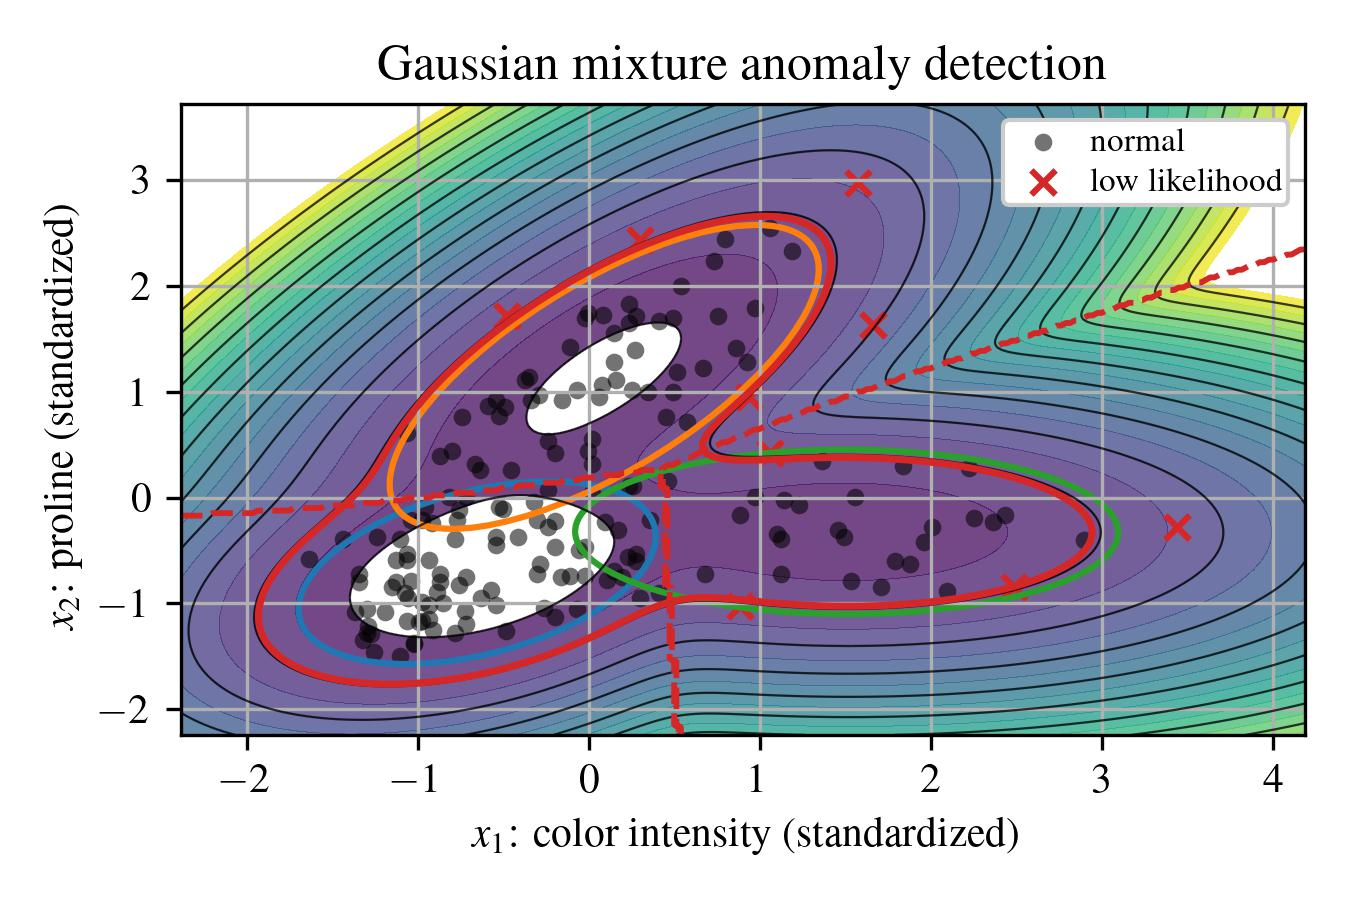
\includegraphics[width=4.5in]{../figures/Gaussian_anomaly_detection}
	\caption{Gaussian mixture anomaly detection applied to the wine data. Observations in low-likelihood regions of the fitted mixture model are flagged as potential anomalies.}
	\label{fig:Gaussian_anomaly_detection}
\end{figure}

The threshold \(\tau\) controls the tradeoff between false alarms and missed anomalies. A high threshold labels more observations as anomalous, increasing sensitivity but also increasing false positives. A low threshold labels fewer observations as anomalous, reducing false positives but potentially missing subtle faults. In practice, \(\tau\) may be selected using a validation set, engineering limits, or an assumed contamination rate representing the expected fraction of anomalies.

In scikit-learn, \texttt{sklearn.covariance.EllipticEnvelope} can be used for Gaussian anomaly detection can when the normal data are reasonably Gaussian. More general anomaly detection methods include \texttt{IsolationForest}, \texttt{LocalOutlierFactor}, and \texttt{OneClassSVM}. These methods use different assumptions, but the modeling goal is the same: learn what normal data look like and identify observations that deviate from that structure.

Clustering and anomaly detection are therefore closely related. Clustering asks, ``Which observations belong together?'' Anomaly detection asks, ``Which observations do not belong with the rest?'' Both questions are unsupervised, both depend strongly on the feature representation, and both require careful interpretation. The output of the algorithm should be treated as evidence of structure in the data, not as a final physical explanation. The final step is always to connect the discovered clusters or anomalies back to the engineering system that produced the measurements.



\end{document}

